
\documentclass[openany]{report}



%*************** Basic ***************
\usepackage[english]{babel}  % Sprache Labels
\usepackage[
  colorlinks = true, 
  linkcolor = {blue!60!black}, 
  citecolor = {blue!60!black},
  urlcolor = {blue!50!black}
]{hyperref}        
\usepackage{titlesec}
\titleformat{\chapter}
  {\normalfont\LARGE\bfseries}{\thechapter}{1em}{}
\titlespacing*{\chapter}{0pt}{3.5ex plus 1ex minus .2ex}{2.3ex plus .2ex}




%*************** Importe ***************
\usepackage{graphicx}
\usepackage{epstopdf}
\usepackage{svg}
\graphicspath{{.}{plots/}{images/}} % Ordner in den gesucht werden soll
\usepackage{makecell}




%*************** Literatur ***************
\usepackage{natbib}            % Naturwissenschaftliches BibTex                
\usepackage{placeins}          % Bibliographie FloatBarrier
\setcitestyle{numbers,square}  % Referenz-style
\bibliographystyle{apsrev4-2}  % Physik-paper-style



%*************** Math ***************
\usepackage{amsmath}  % align-Umgebung
\usepackage{chngcntr}
\counterwithout{equation}{chapter}
\usepackage{amssymb}  % \mathbb{N} usw.
\usepackage{bm}       % Vektoren



%*************** TikZ ***************
\usepackage{tikz}
\usetikzlibrary{matrix, fit, backgrounds}

\newcommand{\upF}{
  \tikz[baseline]{
    \fill[draw] (0,0) -- ++(0,1.4ex) ++(-0.35ex,0) -- ++(0.7ex,0) -- ++(-0.35ex,0.7ex) -- ++(-0.35ex,-0.7ex) -- ++(0.35ex,0)
  }
}

\newcommand{\doF}{
  \tikz[baseline]{
    \fill[draw] (0,0) -- ++(-0.35ex,0.7ex) -- ++(0.7ex,0) -- (0,0) -- ++(-0.35ex,0.7ex) -- ++(0.35ex,0) -- ++(0,1.4ex)
  }
}

\newcommand{\upE}{
  \tikz[baseline]{
    \draw (0,0) -- ++(0,1.4ex) ++(-0.35ex,0) -- ++(0.7ex,0) -- ++(-0.35ex,0.7ex) -- ++(-0.35ex,-0.7ex) -- ++(0.35ex,0)
  }
}

\newcommand{\doE}{
  \tikz[baseline]{
    \draw (0,0) -- ++(-0.35ex,0.7ex) -- ++(0.7ex,0) -- (0,0) -- ++(-0.35ex,0.7ex) -- ++(0.35ex,0) -- ++(0,1.4ex)
  }
}




%******************** Title ********************
\title{
        {\includesvg[scale=1.5]{images/logo.svg}} \\
        \vspace{1cm}
        {\large Bachelor Thesis} \\ 
        {Ising model on a square lattice with competing nearest and next-nearest neighbor interactions} \\
        {\large  Institut für Theoretische Physik Leipzig} \\
        \vspace{7cm} 
        \begin{table}[b]
          \begin{tabular}{ll}
            \multicolumn{2}{l}{\footnotesize{Eingereicht am 17. September 2024}} \\
            \multicolumn{2}{l}{} \\
            1. Gutachter: & Prof. Dr. Wolfhard Janke \\
            2. Gutachter: & Denis Gessert \\
          \end{tabular}
        \end{table}
      } 
\author{Kaspar Mitte \\ Matrikelnummer: 3704209}
\date{}
%************************************************



%**********************************************************************
\begin{document} %*****************************************************
\pagenumbering{gobble} %***********************************************
\maketitle %***********************************************************
%**********************************************************************



\newpage

\subsection*{Eigenständigkeitserklärung}
Hiermit erkläre ich, dass ich die vorliegende Arbeit selbstständig eigenhändig sowie ohne unerlaubte fremde Hilfe und ausschließlich 
unter Verwendung der aufgeführten Quellen und Hilfsmittel angefertigt habe.\\
\\
Leipzig, den 17.09.2024 \\
\begin{tabular}{m{4cm}}
  \\
  \\
  \\
  \hline
  \footnotesize{Kaspar Mitte}
\end{tabular}

\newpage

\begin{abstract}
The Ising model on a square lattice with competing nearest and next-nearest neighbor interactions is highly frustrated for $J_2\!=\!-|J_1|/2$. Further,
the nature of the low temperature behavior is recently under debate. Some authors presume no phase transition at finite temperature 
with different kinds of correlation length divergence~\cite{Kalz2008,Lee2024}. Timmons et al. suggest a glass transition, based on 
computer simulation studies with a single spin update algorithm~\cite{Timmons2018}. This thesis examines the mentioned presumptions by 
studying the specific heat and the spin autocorrelations with an alternative simulation algorithm. The studies of the specific heat with the 
alternative algorithm support an exponential divergence of the correlation length at zero temperature.  A glassy behavior could be observed with 
the single spin update as well. However, it collapses for the alternative update algorithm and is perhaps a dynamic effect. 


\end{abstract}

\newpage

\tableofcontents

\pagenumbering{arabic}

\chapter{Introduction}

  


A while ago, some controversies about spin glasses appeared in the condensed matter physics and statistical physics communities. Under discussion 
were the requirement of quenched disorder, i.e., an explicit dependence on randomness, or whether only frustration is urgently needed as it is for 
structural glasses. Therefore, similarities were presumed between these two kinds of glasses, turned out to be true for some systems. Further, a 
connection between structural glasses and regular magnetic system were closed.

A possible representative of such a system is the frustrated Ising model on a square lattice with competing nearest and next-nearest neighbor interactions.
This model is subjected to significant changes of the ground-state, depending on the ratio of the nearest and next-nearest neighbor interaction. 
The point where these two regimes collide covers a small range around a numerical value of the interaction ratio. In this thesis, this range will 
be denoted as point for simplicity. Further, these regimes exhibit different kinds of ground state patterns (ferromagnetic and super-antiferromagnetic) 
and different kinds of phase transition (continuous and discontinuous), both regimes become 
continuous with enlarging distance to the point of colliding~\cite{Kalz2008,Jin2012,Yoshiyama2023}. The nature of the low temperature phase at the colliding point remains an open question. However, 
it is known that at this point the system is subjected to a high frustration, i.e., it effectively freezes into a metastable state. Kalz et al. developed a 
simulation algorithm in particular for this case, to overcome the high frustration~\cite{Kalz2008}. Timmons et al. propose the high frustration is an 
evidence for glassy behavior~\cite{Timmons2018}. The focus of this thesis is to observe any glassy behavior with the mentioned simulation algorithm.  

This work is structured as follows. Firstly, the physical background is covered from the definition of the considered model and its properties to the 
statistical physics treatment, Chapter~\ref{cha:physics}. Chapter~\ref{cha:methods} contains all used methods for the computer simulation and the 
corresponding data analysis. After that, the procedure of data collection is explained and the associated data is presented and connected to the 
statistical physics properties, Chapter~\ref{cha:results}. Finally, the findings are summarized, and some outlooks are given in 
Chapter~\ref{cha:conclusion}. The Appendix contains the implementation detail, the compiling and execution instructions and some consistency checks. 




\chapter{System under consideration}

  \label{cha:physics}


The model treated is a variation of the conventional Ising model in two dimensions with nearest neighbor interactions 
(NN-interactions). In this work, the next nearest neighbor interactions (NNN-interactions) are additionally considered. 
Therefore, the Hamiltonian is given by 
\begin{align}
    \mathcal{H}(\bm{\sigma})=-J_1\sum_{\langle ij \rangle}\sigma_i\sigma_j-J_2\sum_{[ij]}\sigma_i\sigma_j,
    \label{align:Hamiltonian}
\end{align}
where $\bm{\sigma}\!\in\!\{-\!1,1\}^N$ denotes the microstate with $N$ spins, $\sigma_i$ the components of $\bm{\sigma}$, 
$J_1\!>\!0,J_2\!<\!0$ are coupling constants, $\langle ij \rangle$ denotes the NN-interactions and $[ij]$ the NNN-interactions. The 
studies in this thesis are limited to square lattices with periodic boundary conditions, therefore the total number of spins in a system with 
the lattice length $L$ is $N\!=\!L^2$. 


\section{Ground-state properties}
\label{sec:GroundState}

During the discussion of the ground-state properties of the system described above, Timmons et al. refer in their work~\cite{Timmons2018} to a paper 
of Fan and Wu~\cite{Fan1970} from 1969, containing quite a general analysis of ground-state properties of the vertex model for different 
cases. They mention that for $J_2\in(-\!J_1/2,0]$, the system has a ferromagnetic ground-state, i.e., that all $\sigma_i$ are  either $+\!1$ or $-\!1$. 
To determine the ground-state energy consider the left lattice in Figure~\ref{fig:system1}. 
\begin{figure}[!h]
    \centering
        

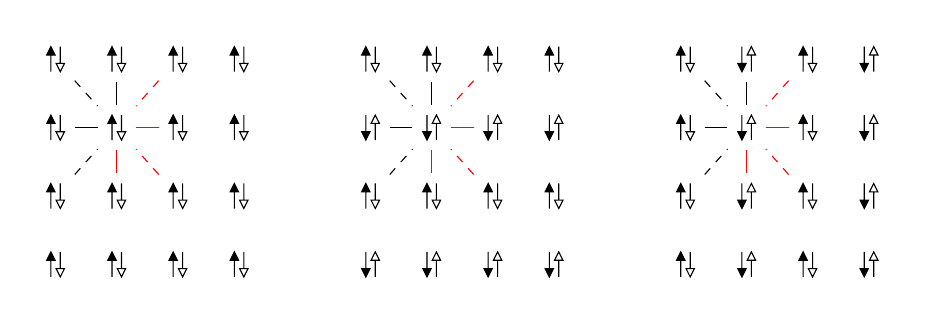
\begin{tikzpicture}
        \matrix[
            matrix of math nodes,
            matrix anchor=west,
            row sep=2ex,
            column sep=2ex,
            ] (m1) at (0,0)
            {
                \upF\doE & \upF\doE & \upF\doE & \upF\doE \\
                \upF\doE & \upF\doE & \upF\doE & \upF\doE \\
                \upF\doE & \upF\doE & \upF\doE & \upF\doE \\
                \upF\doE & \upF\doE & \upF\doE & \upF\doE \\                        
            };
            \path[draw=black]   (m1-1-1) edge[dashed]    (m1-2-2)
                                (m1-3-1) edge[dashed]    (m1-2-2)
                                (m1-2-1) edge            (m1-2-2)
                                (m1-1-2) edge            (m1-2-2)                                                        
            ;
            \path[draw=red]     (m1-1-3) edge[dashed]    (m1-2-2)
                                (m1-3-3) edge[dashed]    (m1-2-2)
                                (m1-2-3) edge            (m1-2-2)
                                (m1-3-2) edge            (m1-2-2)                                                                
            ;

            \matrix[
                matrix of math nodes,
                matrix anchor=west,
                row sep=2ex,
                column sep=2ex,
                ] (m2) at (4,0)
                {
                    \upF\doE & \upF\doE & \upF\doE & \upF\doE \\
                    \doF\upE & \doF\upE & \doF\upE & \doF\upE \\
                    \upF\doE & \upF\doE & \upF\doE & \upF\doE \\
                    \doF\upE & \doF\upE & \doF\upE & \doF\upE \\                         
                };
                \path[draw=black]   (m2-1-1) edge[dashed]    (m2-2-2)
                                    (m2-3-1) edge[dashed]    (m2-2-2)
                                    (m2-2-1) edge            (m2-2-2)
                                    (m2-1-2) edge            (m2-2-2)                                                        
                ;
                \path[draw=red]     (m2-1-3) edge[dashed]    (m2-2-2)
                                    (m2-3-3) edge[dashed]    (m2-2-2)
                                    (m2-2-3) edge            (m2-2-2)
                                    (m2-3-2) edge            (m2-2-2)
                ; 
                \matrix[
                    matrix of math nodes,
                    matrix anchor=west,
                    row sep=2ex,
                    column sep=2ex,
                    ] (m3) at (8,0)
                    {
                    \upF\doE & \doF\upE & \upF\doE & \doF\upE \\
                    \upF\doE & \doF\upE & \upF\doE & \doF\upE \\
                    \upF\doE & \doF\upE & \upF\doE & \doF\upE \\
                    \upF\doE & \doF\upE & \upF\doE & \doF\upE \\                         
                    };
                    \path[draw=black]   (m3-1-1) edge[dashed]    (m3-2-2)
                                        (m3-3-1) edge[dashed]    (m3-2-2)
                                        (m3-2-1) edge            (m3-2-2)
                                        (m3-1-2) edge            (m3-2-2)                                                        
                    ;
                    \path[draw=red]     (m3-1-3) edge[dashed]    (m3-2-2)
                                        (m3-3-3) edge[dashed]    (m3-2-2)
                                        (m3-2-3) edge            (m3-2-2)
                                        (m3-3-2) edge            (m3-2-2)
                    ;   
\end{tikzpicture}
    \caption{ 
                The sketch shows the possible ground-state patterns (left) for $J_2\in(-\!J_1/2,0]$, (middle) and (right) for 
                $J_2\in(-\!\infty,-\!J_1/2)$. The solid lines represent the NN-interactions and the dashed ones the 
                NNN-interactions. 
            }
    \label{fig:system1}
\end{figure}
Each bond drawn contributes $\pm1$ to the sums in the Hamiltonian~\eqref{align:Hamiltonian}, they all are $+\!1$ in the case depicted. To avoid double
summations, sum only over the bonds drawn red for each lattice site. Therefore, one obtains the ground-state energy through a 
summation over the whole lattice $$E_0=\sum_{i=1}^{N}\left( -J_1\cdot2-J_2\cdot2 \right)=-2N(J_1+J_2).$$
For $J_2\in(-\!\infty,-\!J_1/2)$, the system has a super-antiferromagnetic ground-state~\cite{Timmons2018}. Thus, the spins order in
striped patterns of alternating spin values, shown in Figure~\ref{fig:system1} (middle and right lattice). The ground-state energy 
of these four possible states can be computed analogously to the previous case, with the difference that the NN-interactions cancel out for 
each lattice site. Hence, the ground-state energy is given by $$E_0=\sum_{i=1}^{N}\left( -J_1\cdot(1-1)-J_2\cdot(-2) \right)=2NJ_2.$$

Comparing these two ground-state energies, one obtains a special case for $J_2=-\!\frac{J_1}{2}$ because then, the two energy-levels 
coincide. This value of $J_2$ separates these two ground-state regimes, called in the following critical point. At the critical point, the system 
has more than the six ground-states of Figure~\ref{fig:system1}. To obtain the other ground-states, regard
the sketches in Figure~\ref{fig:system2}. Flipping the highlighted lines of aligned spins in the sketched environment, the energy of the 
system does not change.   
\begin{figure}[!h]
    \centering
        

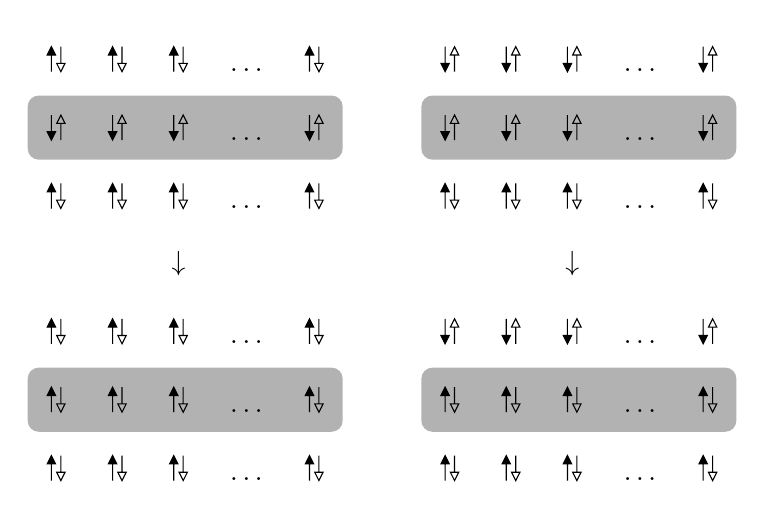
\begin{tikzpicture}
    \matrix[
        matrix of math nodes,
        matrix anchor=west,
        row sep=2ex,
        column sep=2ex,
        ] (m1) at (0,0)
        {
            \upF\doE & \upF\doE & \upF\doE & \dots & \upF\doE \\
            \doF\upE & \doF\upE & \doF\upE & \dots & \doF\upE \\
            \upF\doE & \upF\doE & \upF\doE & \dots & \upF\doE \\
                &     & \downarrow & \\ 
            \upF\doE & \upF\doE & \upF\doE & \dots & \upF\doE \\
            \upF\doE & \upF\doE & \upF\doE & \dots & \upF\doE \\
            \upF\doE & \upF\doE & \upF\doE & \dots & \upF\doE \\                  
        };
    \matrix[
        matrix of math nodes,
        matrix anchor=west,
        row sep=2ex,
        column sep=2ex,
        ] (m2) at (5,0)
        {
            \doF\upE & \doF\upE & \doF\upE & \dots & \doF\upE \\
            \doF\upE & \doF\upE & \doF\upE & \dots & \doF\upE \\
            \upF\doE & \upF\doE & \upF\doE & \dots & \upF\doE \\
                &     & \downarrow & \\ 
            \doF\upE & \doF\upE & \doF\upE & \dots & \doF\upE \\
            \upF\doE & \upF\doE & \upF\doE & \dots & \upF\doE \\
            \upF\doE & \upF\doE & \upF\doE & \dots & \upF\doE \\                    
        };
        \begin{scope}[on background layer]
            \node[fit=(m1-2-1)(m1-2-5), fill=white!70!black, rounded corners] {};
            \node[fit=(m1-6-1)(m1-6-5), fill=white!70!black, rounded corners] {};
            \node[fit=(m2-2-1)(m2-2-5), fill=white!70!black, rounded corners] {};
            \node[fit=(m2-6-1)(m2-6-5), fill=white!70!black, rounded corners] {};            
        \end{scope}                                                             
        ; 
\end{tikzpicture}
    \caption{ 
                The sections of horizontal ground-state patterns for the system at the critical point are depicted. The highlighted rows correspond 
                to the lines that are getting flipped.  
            }
    \label{fig:system2}
\end{figure}
To see that, let $E_{\mathrm{new}/\mathrm{old}}$ be the part of the energy, the highlighted line contributes to. For the left sketch
in Figure~\ref{fig:system2} 
\begin{align*}
    E_\mathrm{new}-E_\mathrm{old}&=(-J_1L\!\cdot\!(2-2)-J_2L\!\cdot\!(-4))-(-J_1L\!\cdot\!4-J_2L\!\cdot\!4)\\
                                 &= -2J_1L-(-2J_1L)=0
\end{align*}
holds. For the right graphic one obtains
\begin{align*}
    E_\mathrm{new}-E_\mathrm{old}&=(-J_1L\!\cdot\!(3-1)-J_2L\!\cdot\!(2-2))-(-J_1L\!\cdot\!(3-1)-J_2L\!\cdot\!(2-2))\\
                                 &= -2J_1L-(-2J_1L)=0.
\end{align*}
Hence, the two processes do not change the energy of the system and one can construct with these two line flips a total of $2^L$ other
ground-states. For the vertical pattern one can construct in an analogous way $2^L$ ground-states, as well. Both cases contain the ferromagnetic 
ground-states, therefore the total number of ground-states generated has to be subtracted by $2$, finally leading to a degeneracy of 
$2^{L+1}\!-\!2$~\cite{Kalz2008}.




  

\section{Statistical physics treatment}
\label{sec:statistical_physics}

In this work the system under consideration is coupled with the environment through an exchange of energy, but not of particles.
Hence, the statistical equilibrium properties of the microstates can be described by the canonical ensemble, i.e., $\bm{\sigma}$ occurs at 
an environment temperature $T$ with a probability 
\begin{align} 
    P(\bm{\sigma})=Z_T^{-1}\exp\left(-\frac{\mathcal{H}(\bm{\sigma})}{kT}\right).
    \label{align:canonical_distribution}
\end{align}
where $Z_T\!\!=\!\!\sum_{\bm{\sigma}}\exp(-\mathcal{H}(\bm{\sigma})/kT)$ denotes the partition function and $k$ the Boltzmann constant. Therefore, 
the expectation value of an arbitrary observable $\mathcal{O}$ depends only on the temperature $T$ and its thermodynamic expectation value
can be computed by
\begin{align*}
    \langle \mathcal{O} \rangle = \sum_{\bm{\sigma}}\mathcal{O}(\bm{\sigma})P(\bm{\sigma}).
\end{align*}
The equilibrium treatment through the canonical ensemble requires the ergodicity, i.e., the expectation value $\langle \mathcal{O} \rangle_\text{time}$ 
obtained through the time evolution of the system coincides with $\langle \mathcal{O} \rangle_\text{phase space}$ received through the geometry of the 
phase space (Ergodic Theorem), in particular its energy surface. Or in more ingenuous words, the system reaches every microstate on the energy 
surface within a sufficiently long duration.~\cite{Landau1976,Schwabl2000} Therefore, Equation~\eqref{align:canonical_distribution} describes
only the thermodynamic equilibrium where the probabilities are independent of the trajectory in the phase space, which in general is not always the case.

Performing the summation over all possible microstates $\sum_{\bm{\sigma}}$ is generally difficult in practice. The density of states delivers a 
concept, to overcome this difficulty. For explanation, let's consider the possible eigenvalues of the Hamiltonian $E\!=\!\mathcal{H}(\bm{\sigma})$ and 
the possible eigenvalues of a microstate dependent observable $M\!=\!\mathcal{M}(\bm{\sigma})$. The density of states $\Omega(E,M)$ assigns 
the number of corresponding microstates to the values $E$ and $M$. The expectation value of observables depending on $E$ and $M$,
can then be rewritten as
\begin{align*}
    \langle \mathcal{O} \rangle = Z_T^{-1}\sum_{E,M}\mathcal{O}(E,M)\Omega(E,M)\exp\left(-\frac{E}{kT}\right).
\end{align*}
Thus, the observable implicitly depends on the microstates $\bm{\sigma}$. To avoid handling with a density of states depending on $E$ and $M$, a
dependency reduction can be performed through $\Omega(E)\!=\!\sum_{M}\Omega(E,M)$. To compute the above expectation value, an effective
energy dependent observable is necessary, received by
\begin{align}
    \langle \mathcal{O} \rangle &= Z_T^{-1}\sum_{E}\frac{\sum_M\mathcal{O}(E,M)\Omega(E,M)}{\sum_M\Omega(E,M)}\Omega(E)\exp\left(-\frac{E}{kT}\right) \nonumber \\
                                &= Z_T^{-1}\sum_{E}\mathcal{O}_\text{eff}(E)\Omega(E)\exp\left(-\frac{E}{kT}\right).
    \label{align:Lists}
\end{align}
The effective observable $\mathcal{O}_\text{eff}(E)$ is also known as list, an actual energy
dependency of $\mathcal{O}(E,M)$ is not required. Further, $\mathcal{O}_\text{eff}(E)$ is the expectation value of $\mathcal{O}(\bm{\sigma})$ with 
$\bm{\sigma}$ distributed according to the micro canonical ensemble (no $E$ exchange). This reduction procedure works with any observable $M$.~\cite{Janke2012}





\subsection*{Thermodynamic quantities}

To treat the studied thermodynamic quantities properly, consider the Hamiltonian~\eqref{align:Hamiltonian} with a non-vanishing external magnetic 
field $h$ aligned parallelly to the spins $\sigma_i$
\begin{align*}
    \mathcal{H}_h(\bm{\sigma})=-J_1\sum_{\langle ij \rangle}\sigma_i\sigma_j-J_2\sum_{[ij]}\sigma_i\sigma_j+h\sum_{i=1}^N\sigma_i.
\end{align*}
For simplicity, let $\mathcal{M}(\bm{\sigma})$ denotes the microstate dependent sum $\sum_{i=1}^N\sigma_i$. Using the modified Hamiltonian, define 
the thermodynamic potential
\begin{align}
    F(T,h)=-kT\ln\left(Z_{T,h}\right)=-kT\ln\left(\sum_{\bm{\sigma}}\exp(-\mathcal{H}_h(\bm{\sigma})/kT)\right),
    \label{align:FreeEnergy}
\end{align}
also known as canonical free energy. Its partial derivatives are given by
\begin{align}
    \partial_TF(T,h) &= -k\ln\left(Z_{T,h}\right)-\frac{kT}{Z_{T,h}} \sum_{\bm{\sigma}}\frac{\mathcal{H}_h(\bm{\sigma})}{kT^2}\exp\left(-\frac{\mathcal{H}_h(\bm{\sigma})}{kT}\right) \nonumber \\
                     &= -k\ln\left(Z_{T,h}\right)-\frac{\left\langle E \right\rangle}{T} \label{align:ener} \\
    \partial_hF(T,h) &= \frac{kT}{Z_{T,h}}\sum_{\bm{\sigma}}\frac{\partial_h\left(\mathcal{H}(\bm{\sigma})+h\mathcal{M}(\bm{\sigma})\right)}{kT}\exp\left(-\frac{\mathcal{H}_h(\bm{\sigma})}{kT}\right) \nonumber \\
                     &= -\left\langle M \right\rangle, \label{align:magn}
\end{align}
where the non-respected macroscopic state variables are kept fixed. Especially, both the internal energy $\left\langle E \right\rangle$ 
and the conventional magnetization\footnote{The term conventional is used, because some modified magnetizations are defined in the following.} 
$\left\langle M \right\rangle$ can be obtained through partial derivatives of the free energy $F$. 
Furthermore, the internal energy is a function received via a Legendre-transformation~\cite[p.79]{Schwabl2000} of the free energy, i.e., 
$\left\langle E \right\rangle\!(\partial_TF,h)=T\partial_TF(T,h)\!-\!F(T,h)$. Other relevant thermodynamic quantities are the specific heat $c_V$ and
susceptibility $\chi$ defined as the second partial derivatives of the free energy 
\begin{align}
    c_V  \!&=\! -\frac{T\partial_T^2F(T,h)}{N} 
          = \frac{T}{N}\left( - \frac{k}{Z_{T,h}}\!\sum_{\bm{\sigma}}\frac{\mathcal{H}_h(\bm{\sigma})}{kT^2}\exp\left(-\frac{\mathcal{H}_h(\bm{\sigma})}{kT}\right) 
                              + \frac{\langle E \rangle}{T^2} + \frac{\partial_T\langle E \rangle}{T}\right) \nonumber \\
         &= \frac{\sum_{\bm{\sigma}}\mathcal{H}_h(\bm{\sigma})\partial_T\exp\left(-\mathcal{H}_h(\bm{\sigma})/kT\right)}
                 {NZ_{T,h}}
           -\frac{\langle E \rangle\sum_{\bm{\sigma}}\partial_T\exp\left(-\mathcal{H}_h(\bm{\sigma})/kT\right)}
                 {NZ_{T,h}} \nonumber \\
         &= \frac{\langle E^2 \rangle-\langle E \rangle^2}{NkT^2}  \label{align:heat} \\
    \chi &= -\frac{\partial_h^2F(T,h)}{N} = \frac{\partial_h\langle M \rangle}{N} \nonumber \\
         &= \frac{\sum_{\bm{\sigma}}\mathcal{M}(\bm{\sigma})\partial_h\exp\left(-\mathcal{H}_h(\bm{\sigma})/kT\right)}
                 {NZ_{T,h}}
           -\frac{\langle M \rangle\sum_{\bm{\sigma}}\partial_h\exp\left(-\mathcal{H}_h(\bm{\sigma})/kT\right)}
                 {NZ_{T,h}} \nonumber \\
         &= \frac{\langle M^2 \rangle-\langle M \rangle^2}{NkT}. \label{align:susc} 
\end{align}
Therefore, the internal energy, conventional magnetization, specific heat and susceptibility can be expressed both in terms of partial derivatives of a 
thermodynamic potential  and in terms of expectation values. This fact justifies the importance of these observables for critical phenomena studies with 
computer simulations.~\cite{Schwabl2000}

The quantities above are these for a non-vanishing external field. Taking the limit $\lim_{h\to0}\mathcal{O}$ corresponding to 
$\mathcal{H}_h,Z_{T,h}\to\mathcal{H},Z_T$, the quantities are obtained for $h\!=\!0$.  





\section{Phase transition}
\label{sec:phase_transitions}

In thermodynamics there exists critical phenomena so-called phase transitions, where the system is subjected to significant property changes. Such 
transitions occur through changes in the symmetry of the system, i.e., changes to a state of more (or less) symmetry or changes between different unrelated 
symmetries~\cite{Landau1976}. The different states are called phases, the state with the lower symmetry is named ordered phase, as opposed to the 
disordered phase of higher symmetry. The engine of such transitions are variations of the macroscopic state variables. In the considered case 
these are the temperature $T$ and the external magnetic field $h$. To describe these phenomena quantitatively, an order parameter is commonly used, 
assigning to the ordered phase a finite value and vanishing for the disordered one. More generally, the order parameter is finite at one of the phases 
and vanishes at the other one, but such an order parameter does not always exist.~\cite{Landau1976,Schwabl2000}

For the system under consideration, a quantity of high interest is the two point spin correlation function
\begin{align*}
    G(i,t_1,j,t_2)=\langle \sigma_i(t_1)\sigma_j(t_2) \rangle - \langle \sigma_i(t_1) \rangle\langle \sigma_j(t_2) \rangle,
\end{align*}
where $t_1,t_2$ denotes two times in system history. To achieve a better understanding of this function, let's consider the term 
$1\!+\!\langle \sigma_i(t_1)\sigma_j(t_2) \rangle$, which is proportional to the probability of observing the $i^\text{th}$ spin at $t_1$
aligned equally to the $j^\text{th}$ spin at $t_2$~\cite{Stanley1987}. Hence, this correlation function evaluates the microscopic relations of the 
system so $G(i,t_1,j,t_2)$ quantifies the correlations between $\sigma_i(t_1)$ and $\sigma_j(t_2)$. The considered system has translation 
invariance, therefore $G$ is actually a function of the delay $j\!-\!i$. Two cases can be examined, firstly, at $t_1\!=\!t_2$, the two point spin correlation
function decays exponentially for large delays $j\!-\!i\gg 1$ according to
\begin{align*}
    G(j\!-\!i)\propto |a\cdot(j\!-\!i)|^{-\kappa}\exp\left(-\frac{a\cdot(j\!-\!i)}{\xi}\right),
\end{align*}
with the lattice constant $a$, a dimension and system dependent exponent $\kappa$ and the spatial correlation length $\xi$ modelling the effective 
affecting range of a spin~\cite{Janke2012}. Secondly, for $j\!-\!i=0$, it is convenient to average the spin values over 
the whole lattice, because no lattice site is preferable under periodic boundary condition. Furthermore, to normalize the resulting expression to unity 
for $t_1\!=\!t_2$ and afterward to take the thermodynamic expectation value. Thus, the general expression of the two point spin correlation function becomes
\begin{align}
    G(t_1,t_2) &= \left\langle \frac{\frac{1}{N}\sum_{i=1}^N\sigma_i(t_1)\sigma_i(t_2)-\frac{1}{N}\sum_{i=1}^N\sigma_i(t_1)\cdot\frac{1}{N}\sum_{i=1}^N\sigma_i(t_2)}
                                    {1-\frac{1}{N}\sum_{i=1}^N\sigma_i(t_1)\cdot\frac{1}{N}\sum_{i=1}^N\sigma_i(t_2)}\right\rangle \nonumber \\
               &= \left\langle \frac{N\sum_{i=1}^N\sigma_i(t_1)\sigma_i(t_2)-\mathcal{M}(\bm{\sigma}(t_1))\mathcal{M}(\bm{\sigma}(t_2))}
                                    {N^2-\mathcal{M}(\bm{\sigma}(t_1))\mathcal{M}(\bm{\sigma}(t_2))}\right\rangle.
    \label{align:spin_correlation}
\end{align}

In a mathematical sense, the free energy $F(T,h)$ is a non-analytical function at the phase transition. Hence, phase transitions can be characterized 
according to the discontinuities of the partial derivatives of $F(T,h)$. A phase transition is called discontinuous if $F(T,h)$ is continuous and at least 
one  of the first derivatives has a discontinuity. A continuous phase transition is classified through a continuous first partial derivatives and singularities
or discontinuities in the higher order.~\cite{Schwabl2000} Of course there are some exotic cases, which cannot be classified in a conventional fashion. It 
should be emphasized that these discontinuities and singularities actually appear for infinite system sizes only in the thermodynamic limit. For finite systems 
the free energy is usually analytical. Only finite system sizes are possible in computer simulation studies. Therefore, the results have to be extrapolated 
to $N\!\to\!\infty$.~\cite{Janke2012}

In the following, the conventional kinds of phase transitions are shortly described, as well as a representative of the exotic ones. Additionally, the discussions
are limited to the temperature driven phase transitions. Thus, the phase transition point is located through a critical temperature $T_c$.





\subsection*{Discontinuous phase transition}

As mentioned, this kind of phase transitions are characterized by discontinuous changes of the first partial derivative of the free energy. Hence, discontinuities
in the entropy $S\!=\!-\partial_TF(T,h)$ or magnetization $\langle M\rangle\!=\!-\partial_hF(T,h)$ suggest $\delta$-function singularities of the specific heat
or the susceptibility. The free energy is reflected by two different analytical functions
$F_1(T,h)$ for $T\!<\!T_c$ and $F_2(T,h)$ for $T\!>\!T_c$, satisfying the continuity condition $F_1(T_c,h)\!=\!F_2(T_c,h)$ at the transition point. 
Each function corresponds to a phase~\cite{Landau1976}. Thus, the 
transition point exhibits a coexisting state of both phases, implying a finite spatial correlation length $\xi$, i.e., there are finite regions 
corresponding to the phases  involved. In simulation studies, such phenomena are noticeable by double-peaked energy or magnetization histograms,
where each peak corresponds to one of the phases.~\cite{Janke2003}

The considered system is subjected to a discontinuous phase transition for $J_2/J_1\!\in\!(-g^*,-1/2)$ with $g^*\!\approx\!0.67$~\cite{Jin2012}, which is 
still under debate. This
critical behavior is supported by the work of Kalz et al.~\cite{Kalz2008} as well. Especially, they obtain the double-peaked histograms and argue
for a $\delta$-function singularity of the specific heat in the thermodynamic limit. For this case, the ground-states are super-antiferromagnetic as pointed 
out in Section~\ref{sec:GroundState}. This justifies the following choice of the order parameter
\begin{align}
    \mathcal{M}_s(\bm{\sigma}) = \begin{cases}
                                    \mathcal{M}_h(\bm{\sigma})=\sum_{i=1}^N(-1)^{x_i}\sigma_i & \text{for } |\mathcal{M}_h|>|\mathcal{M}_v| \\
                                    \mathcal{M}_v(\bm{\sigma})=\sum_{i=1}^N(-1)^{y_i}\sigma_i & \text{for } |\mathcal{M}_h|\le|\mathcal{M}_v|
                                 \end{cases}
    \label{align:stripped_magnetization}
\end{align}
where $x_i,y_i\!\in\!\{1,...,L\}$ index the columns and rows of the lattice. $\mathcal{M}_s$ assigns the super-antiferromagnetic ground-states with 
$\pm N$ and effectively vanishes for spin configurations distributed uniformly (corresponding to the high temperature phase). Furthermore, 
$\langle M_{s,h,v}\rangle$ can be considered as modified magnetizations and all previous expressions of quantities containing the conventional magnetization 
can be adjusted by replacing $\mathcal{M}$ with $\mathcal{M}_{s,h,v}$, like Equations~\eqref{align:susc} and~\eqref{align:spin_correlation}. 
In the following, the index $s,h,v$ is related to this very replacement. 





\subsection*{Continuous  phase transition}

The phase transitions of continuous kind have at least continuous changes of the free energy and their first partial derivatives. The ones being discontinuous
in their second derivatives in form of singularities have a major status and are being examined in the following. The corresponding free energy can be expressed 
by a single continuously differentiable function describing both phases. Therefore, the transition point exhibits a continuous mixture containing the symmetries 
of both phases, i.e., there is no coexisting of finite regions corresponding to the different phases and rather a single "transition phase" subjected to the whole 
system.~\cite{Landau1976,Schwabl2000} Hence, the spatial correlation length diverges $\xi\!\to\!\infty$ at $T_c$, according to the power law
$$ \xi \propto\left|1-T/T_c\right|^{-\nu}+\Delta_\xi, $$
where $\nu$ denotes a characteristic exponent also known as the critical exponent and $\Delta_\xi$ is a correction term. The 
singularities of the second partial derivatives of $F(T,h)$ and the order parameter (for the magnetic systems, $\langle M \rangle$) behaves according to 
power laws in the vicinity of $T_c$ as well,
$$ c \propto \left|1-T/T_c\right|^{-\alpha}+\Delta_c,$$
$$ \langle M \rangle \propto \left(1-T/T_c\right)^{\beta}+\Delta_M \  \text{ for } \  T<T_c, $$
$$ \chi \propto \left|1-T/T_c\right|^{-\gamma}+\Delta_\chi, $$
with the critical exponents $\alpha,\beta,\gamma$ and the correction terms $\Delta_{(\cdot)}$.~\cite{Janke2012} The possible values of the exponents 
$\alpha,\beta,\gamma,\nu$ define the universality of critical phenomena, i.e., in proximity of $T_c$, the microscopic details of the interactions becomes 
irrelevant and only universal properties, like dimension, symmetry of the order parameter or general character of the interaction are essential. 
Therefore, different systems with the same universal properties behave equally in the vicinity of $T_c$. These facts are supported by the renormalization
group theory.~\cite{Schwabl2000} In computer simulation studies, it is impossible to observe actual divergences, because only finite system sizes are 
possible such that the singularities appear rather as dislocated and rounded peaks, and it is necessary to extrapolate the finite size observations
to an infinite system size (thermodynamic limit). This can be done with the finite-size scaling approach $\xi\to L$, where $L$ is the linear system size 
(lattice length), implying the relation
\begin{align}
    \left|1-T/T_c\right| \propto L^{-1/\nu}.
    \label{align:FSS_power}
\end{align}
For finite systems the spatial correlation length is limited by $L$, justifying the replacement of $\xi$ with large $L$.~\cite{Janke2012} 

The discussion above holds for a huge number of systems but in some cases the phase transition exhibits a continuous character and a different spatial
correlation length divergence, i.e., the power law divergence of $\xi$ is not strong enough, causing an exponential divergence
\begin{align*}
    \xi \propto \exp\left(c\left| 1-T/T_c \right|^{-\overline{\nu}}\right) + \Delta_\xi,
\end{align*}
with some system dependent constant $c$ and a new exponent $\overline{\nu}$. Similarly, the finite-size approach can be followed according to the replacement 
of $\xi$ with large $L/L_0$, leading to the relation
\begin{align}
    \left|1-T/T_c\right| \propto \left( \ln\left(L/L_0\right)\right)^{-1/\overline{\nu}},
    \label{align:FSS_exponential}
\end{align}
with a system dependent characteristic length scale $L_0$. This idea is originated by a work of Kosterlitz~\cite{Kosterlitz1974}, studying the 
two-dimensional XY-model ($\overline{\nu}=1/2$).

Back to the considered system of this thesis, different papers~\cite{Kalz2008,Landau1980,Li2021} point out that the kind of the phase transition is 
continuous for the system with $J_2/J_1\!\in\!(-1/2,0]$. The corresponding order parameter is the conventional magnetization $\mathcal{M}(\bm{\sigma})$. 
Furthermore, they found the same set of critical exponents as the conventional Ising model ($J_2/J_1=0$), suggesting
a membership of the Ising universality class. Hence, all mentioned variations of the considered system behave equally in proximity of there 
respective transition point. It should be emphasized that the critical exponents are equal but the transition temperatures $T_c$ differ. 





\subsection*{Glassy phase transition}

These kinds of phase transition are subjects of recent researches. There are dynamical and static approaches to treat these phase transitions in the context 
of statistical physics. In the low temperature phase, the difficulty of this kind originates from the non-ergodic behavior and the huge number of deep free 
energy valleys (metastable states), i.e., the system is easily trapped in a sub-state space and effectively freezes in this state. 
Especially, the states minimizing the free energy in the state space have a random character, thus the corresponding microstates have no significant 
similarities and appear disordered or asymmetrical (no ordered patterns in a conventional sense such as the ferromagnetic or super-antiferromagnetic ones). 
Usually, the freezing into a metastable state results from competing interactions. Conventionally, the term 
"glassy" is distinguished in spin glasses and structural glasses.~\cite{Binder1986,Mezard2000}

A spin glass is commonly characterized by freezing into a metastable state and quenched disorder, i.e., the system depends 
explicitly on random variables that are independent of time on all experimental
time scales~\cite{Binder1986}. In context of spin glasses the freezing property is also known as
frustration. The latter property can be explained by the Edwards-Anderson model defined as the Hamiltonian
\begin{align*}
    \mathcal{H}(\bm{\sigma})=-\sum_{\langle ij \rangle}J_{ij}\sigma_i\sigma_j,
\end{align*}
with Gaussian-distributed $J_{ij}$. The thermodynamic quantities of interest are obtained through their averages over different system realizations 
corresponding to a set of $J_{ij}$ drawn randomly, also known as replica. Hence, the disordered appearance of the metastable states or "random-valleys"
in the free energy results from explicit random variables in the Hamiltonian.~\cite{Binder1986} However, some newer publications, like 
Ref.~\cite{Westfahl2001,Kamber2020}, argue for spin glass without quenched disorder, i.e., self generated randomness.



A structural glass effectively freezes into an unsymmetrical microstate as well, denoted in this context as an amorphous state. However, their origin is 
different, the randomness or disorder of the metastable states is self generated like the arrangement of the atomic bonds in chemical glass. Therefore, the 
"random-valleys" characteristic of the free energy is a system related property and less artificial than in spin glasses, i.e., the main difference
to spin glasses is the absence of quenched disorder. Thus, the replicas result from independent system preparations and not from a new set of random 
variables.~\cite{Mezard2000}

Kirkpatrick et al. begin to blur the boundaries between spin glasses and structural glasses in their papers~\cite{Kirkpatrick1986,Kirkpatrick1987},
mentioning analogies between structural glasses and Potts spin glasses. They list similarities to discontinuous phase transitions and 
suggest possible glassy behavior of frustrated regular spin problems. Furthermore, these kinds of
problems are named discontinuous spin glasses, which exhibits a continuous change of the entropy, internal energy and a discontinuous
change of the order parameter~\cite{Mezard2000}. A general theory containing these kinds of problems is developed in a paper of Westfahl et al.~\cite{Westfahl2001}. 

This analytical approach predicts a possible temperature range of the glass transition temperature $T_g$, where the system effectively freezes into a 
metastable state, i.e., $T_g\!\in\!(T_K,T_A)$ with the limit temperatures $T_K,T_A$ of glassy behavior. M\'ezard et al.~\cite{Mezard2000} mention a relaxation 
time $\tau$ divergence of the spin autocorrelations 
at $T_g$ where the explicit value of this temperature depends on the cooling rate~\cite{Westfahl2001}. The lower boundary $T_K$ corresponds to the ideal 
glass transition temperature in the infinite cooling rate limit~\cite{Timmons2018}. A connection between $\tau$ and the limit temperature $T_K$ is
given by the Vogel-Fulcher law~\cite{Kirkpatrick1987,Westfahl2001}
\begin{align}
    \tau\propto\exp\left(\frac{c\cdot T_K}{T-T_K}\right).
    \label{align:Vogel_Fulcher}
\end{align}
The upper boundary $T_A$ exhibits the occurrence temperature of the metastable state~\cite{Kirkpatrick1987}, i.e., 
these states appear with a non-negligible probability, resulting in significantly increasing spin autocorrelations, because the system is subjected to 
strong memory effects.

The nature of the system under consideration for $J_2/J_1\!=-\!1/2$ is unclear in the low temperature range (nonzero $T$). There are some evidence supporting
a glassy behavior depicted above~\cite{Timmons2018}. Firstly, the huge number of metastable states (degeneracy), Section~\ref{sec:GroundState} and the frustration 
arising from the competition between the  NN-term and repulsive NNN-term in the Hamiltonian~\eqref{align:Hamiltonian}. Secondly, discontinuous spin glasses 
have both a continuous and discontinuous character, which may connect the two regimes for $J_2/J_1\!\in\!(-g^*,-1/2)$ and $J_2/J_1\!\in\!(-1/2,0]$.
However, there are also evidences against it, like the absence of the random or disordered characteristic of the metastable states, and 
especially the ordered form of the ground-states~\cite{Kalz2008,Lee2024}.












\chapter{Methods}

  \label{cha:methods}


\section{Monte Carlo simulations}
\label{sec:MCsimulations}

In a statistical physic setup, simulation methods become important either if the enumeration of the microstates reaches a huge number of terms or if there is no 
analytical method to determine the density of states or partition function of the considered system. To overcome these problems, 
sample the time evolution of the system  with fixed macroscopic state variables, i.e., a fixed environment temperature $T$ for the canonical ensemble. 
Hence, the microstates arising should be distributed according to the probability distribution of the canonical ensemble, Equation~\eqref{align:canonical_distribution}, 
(if the system is in equilibrium) and one estimates the expectation value through the given microstates $\bm{\sigma}_k$ where $k$ indexes the $M$ 
measurements. Therefore, an arbitrary observable $\mathcal{O}$ can be estimated by
\begin{align}
    \hat{\mathcal{O}}_T=\frac{1}{M}\sum_{k=1}^M\mathcal{O}(\bm{\sigma}_k)
    \label{align:MCidea}
\end{align}
if $M$ is sufficiently large and the system is properly equilibrated, i.e., the occurrence of the microstates follows the underlying probability 
distribution. To achieve such time evolution of the microstates one can use Markow chain Monte Carlo methods (MCMC methods) originating from the 
work of Metropolis et al.~\cite{Metropolis1953}.

\subsection*{MCMC method}

The idea of MCMC methods is to let the system transit from a microstate $\bm{\sigma}_i$ to $\bm{\sigma}_j$ with a transition probability $W_{ij}$, and 
thus the transition $\bm{\sigma}_i\to\bm{\sigma}_j$ happens with a probability $W_{ij}$ where the case $i\!=\!j$ is allowed as well. To sample the 
underlying distribution, the following requirements for $W_{ij}$ are necessary
\begin{align}
    &W_{ij} \ge 0                        &\forall i,j  
        \label{align:con1}\\
    &\sum_jW_{ij} = 1                    &\forall i
        \label{align:con2}\\
    &W_{ij}P(\bm{\sigma}_i)=W_{ji}P(\bm{\sigma}_j) &\forall i,j
        \label{align:con3}\\
    &\exists\bm{\sigma}_{k_1},...,\bm{\sigma}_{k_n} \  n\!\in\!\mathbb{N} \  \text{  such that} 
                             \sum_{k_1,...,k_n}\!\!\!\!W_{ik_1}\!\!\cdot...\cdot\!W_{k_nj}>0 &\forall i,j.
        \label{align:con4}
\end{align}
Conditions~\eqref{align:con1} and~\eqref{align:con2} ensure the strict positivity and normalization of probabilities. Equation~\eqref{align:con3} is also known as 
detailed balance, implying that a transition $\bm{\sigma}_i\to\bm{\sigma}_j$ is reversible, and hence no directions of the transitions $\bm{\sigma}_i\leftrightarrow\bm{\sigma}_j$ 
is preferred. The balance condition $\sum_iW_{ij}P(\bm{\sigma}_i)=P(\bm{\sigma}_j)$ can easily be obtained by a summation of the detailed balance from which
it follows that the equilibrium probabilities $P(\bm{\sigma}_j)$ are the components of an eigenvector of the transition matrix ($W_{ij}$ can be 
considered as a matrix).
Therefore, the transitions conserve the underlying equilibrium distribution, and it is urgently necessary to equilibrate the system such that the occurrence
of the microstates reflects the equilibrium distribution. Condition~\eqref{align:con4} ensures the ergodicity, i.e., all possible states
can be reached through a finite number of transitions with non-vanishing probability. Thus, no transition traps the system in a sub-state space.~\cite{Janke2012}

In this thesis, all microstate transitions are constructed via the following steps. Firstly, one selects a transition
proposal from $\bm{\sigma}_i$ to $\bm{\sigma}_j$ with probability $f_{ij}$. Secondly, the transition is accepted with a probability $w_{ij}$. Hence, for $i\!\neq\!j$,
the transition probability is  given by $W_{ij}\!=\!f_{ij}w_{ij}$ and by $W_{ii}\!=\!1\!-\!\sum_{n\neq m}\!W_{nm}$ for $i=j$. The acceptance probability
\begin{align*}
    w_{ij}=\min\left\{1,\frac{f_{ji}P(\bm{\sigma}_j)}{f_{ij}P(\bm{\sigma}_i)}\right\}
          =\min\left\{1,\frac{f_{ij}}{f_{ji}}\exp\left(-\frac{\mathcal{H}(\bm{\sigma}_j)-\mathcal{H}(\bm{\sigma}_i)}{kT}\right)\right\}
\end{align*}
then defines the Metropolis algorithm, which indeed
satisfies Condition~\eqref{align:con1},~\eqref{align:con2} and~\eqref{align:con3}.~\cite{Janke2012} 

The ergodicity condition depends on the exact shape of the microstate changing rule. For the numerical work the following two local update algorithms 
are implemented. 



\subsection*{Single spin update algorithm}

In this update method the transition $\bm{\sigma}_i$ to $\bm{\sigma}_j$ results from a single spin flip obviously satisfying Condition~\eqref{align:con4} 
because each possible state can be generated by a finite number of spin flips. Firstly, one chooses a spin at random corresponding
to $f_{ij}=1/N$. Secondly, this spin will be flipped with a probability $w_{ij}=\min\{1,\exp(-\Delta E/kT)\}$, where $\Delta E$ denotes the
energy deviation resulting from flipping the spin. The simulation steps are conventionally measured in sweeps, where one sweep contains $N$ spin flip 
proposals.

The advantage of this compact algorithm is that a huge number of systems can be simulated because a single spin flip can easily be applied to any "Ising like" 
system. However, for frustrated systems at low $T$ the proposals are almost certainly refused and a transition between the free energy minima requires 
a relatively huge number of accepted proposals, thus the system remains in the 
current microstate over a large number of spin flip proposals thereby expanding the simulation time to collect reliable data. Unluckily, the system under consideration 
is such a system, but the following update algorithm could be the solution to this dilemma. 



\subsection*{Line spin update algorithm}

In this update method the microstate transition will be enabled both through a line flip and a single spin flip. A line flip consists of flipping all 
the spins highlighted gray in Figure~\ref{fig:simulation1}. Of course, choosing other rows and columns is possible as well.
\begin{figure}[!h]
    \centering
        

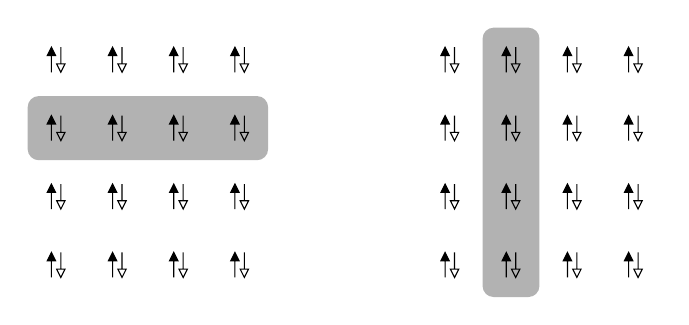
\begin{tikzpicture}
    \matrix[
        matrix of math nodes,
        matrix anchor=west,
        row sep=2ex,
        column sep=2ex,
        ] (m1) at (0,0)
        {
            \upF\doE & \upF\doE & \upF\doE  & \upF\doE \\
            \upF\doE & \upF\doE & \upF\doE  & \upF\doE \\
            \upF\doE & \upF\doE & \upF\doE  & \upF\doE \\
            \upF\doE & \upF\doE & \upF\doE  & \upF\doE \\                 
        };
    \matrix[
        matrix of math nodes,
        matrix anchor=west,
        row sep=2ex,
        column sep=2ex,
        ] (m2) at (5,0)
        {
            \upF\doE & \upF\doE & \upF\doE  & \upF\doE \\
            \upF\doE & \upF\doE & \upF\doE  & \upF\doE \\
            \upF\doE & \upF\doE & \upF\doE  & \upF\doE \\
            \upF\doE & \upF\doE & \upF\doE  & \upF\doE \\                          
        };
        \begin{scope}[on background layer]
            \node[fit=(m1-2-1)(m1-2-4), fill=white!70!black, rounded corners] {};
            \node[fit=(m2-1-2)(m2-4-2), fill=white!70!black, rounded corners] {};            
        \end{scope}                                                             
        ; 
\end{tikzpicture}
    \caption{This Figure shows two line flip proposal of the $2L$ possible ones.}
    \label{fig:simulation1}
\end{figure}
The additional single spin flip is necessary to satisfy Condition~\eqref{align:con4} because by only applying line flips, the entire state space 
cannot be covered. For example, the system is initiated in a nearly ideal ferromagnetic state, with one spin aligned in the opposite direction. 
There exists no sequence of line flips that transits the system from the initial state mentioned to an ideal ferromagnetic state, hence the system is 
trapped in a sub-state space. To apply this update method in practice, firstly choose a line at random of the $2L$ columns and rows with 
a selection probability $f_{ij}=1/2L$. This line will be flipped with a probability $w_{ij}=\min\{1,\exp(-\Delta E/kT)\}$, but now $\Delta E$ results 
from a flipped line. After the line flip proposal one has to perform $L$ spin flip proposals such that $L/2$ repetitions of this procedure correspond 
to one sweep. With this unit of simulation steps, the two depicted update algorithms are comparable. 

The advantage of the modified algorithm is to overcome the high rejection rate in the frustrating temperature range of the system. The line flips 
mentioned in Section~\ref{sec:GroundState} applied to an aligned ground-state cost no energy, therefore the line flips are accepted more frequently
at low $T$ because the system is in a near ground-state and a line flip has low energy costs. This line spin update 
algorithm was first presented in a paper of Kalz et al.~\cite{Kalz2008}




\section{Pseudo random number generators}

In the two previous subsection, the simulation algorithms depicted rely on stochastic experiments, in particular on the randomly
chosen lattice sites or lines and the acceptance of the flip proposals. Even for the smallest considered lattice length, the number 
of such stochastic experiments amounts to many millions. Rolling the dice is definitely not the way to go, performing these stochastic
experiments in a reasonable time. In computer simulation studies, pseudo random number generators (PRNG) overcome
this problem. PRNG are based on some deterministic rule, producing a sequence of numbers $X_i$ with a random face, i.e., $X_i$ appear 
to be drawn randomly. An example of such a deterministic rule is the linear congruential generators defined by the recursive sequence
\begin{align*}
    X_{i+1}=(aX_i+c)\mathrm{mod}(m),
\end{align*}
producing pseudo random numbers between $0$ and $m\!-\!1$, with $a,c,m\!\in\!\mathbb{N}$~\cite{Janke2002}. There are many of such algorithms,
with advantages and disadvantages for their purposes. The main criterions are the period length, i.e., the number of iteration 
until the same sequence returns, and the efficiency in context of the computational workload. Furthermore, some algorithms exhibit a "resonant" 
behavior with some application, i.e., the randomness fails, and unreliable data can be produced~\cite{Janke2002}. Therefore, care is 
necessary for the choice of the PRNG. 

For the numerical work in this thesis, the $32\mathrm{bit}$ Mersenne Twister \verb|mt19937| PRNG of 
the \verb|c++11| standard library is used, which is considered as very well tested and as a common choice for Monte Carlo simulation studies.
Additionally, this PRNG has a very large period length of $2^{19937}\!-\!1$. 

Many of the PRNG and particularly the Mersenne Twister generator produces uniformly distributed integers. An additional step is necessary to obtain 
non-uniform distributed pseudo random number. For explanation, let be $P(x)$ some invertible probability distribution of the random variable $X$ 
and $p\!\in\![0,1)$ a pseudo random number drawn uniformly. Thus, the probability of the event $X\!=\!x^*$ is given by $P(x^*)$. Then, a 
pseudo random number distributed according to $P(x)$ can be obtained through the inversion $x^*\!=\!P^{-1}(p)$.~\cite{Janke2002}






  

\section{Error estimation}
\label{sec:error}

The idea of the simulation method described in Section~\ref{sec:MCsimulations} is to approximate the theoretical expectation value
$\langle \mathcal{O} \rangle$ of a microstate dependent observable $\mathcal{O}(\bm{\sigma})$ through Equation~\eqref{align:MCidea}. This estimate
depends on the number of measurements $M$ and the explicit outcomes of the stochastic experiments, and hence the estimator $\hat{\mathcal{O}}$ carries an error 
and fluctuates around the exact expectation value. One has to chose $M$ properly such that the expense of simulation time and the statistical error of the estimate 
are in balance. A 
quantity to evaluate the deviation between $\hat{\mathcal{O}}$ and $\langle \mathcal{O} \rangle$ is the variance 
\begin{align*}
    \sigma_{\hat{\mathcal{O}}}^2 = \langle \hat{\mathcal{O}}^2\rangle-\langle \hat{\mathcal{O}} \rangle^2.
\end{align*}
In the following, the term "error" refers to the square root of the variance also known as one-sigma-error. If all requirements of
the Central Limit Theorem~\cite[p.246]{Behrends2013} are sufficiently fulfilled, roughly $68\%$ of the independently estimated values will satisfy
$\hat{\mathcal{O}}\!\in\![\langle \hat{\mathcal{O}} \rangle\!-\!\sigma_{\hat{\mathcal{O}}},\langle \hat{\mathcal{O}} \rangle\!+\!\sigma_{\hat{\mathcal{O}}}]$.
The expression of the variance can be rewritten using Equation~\eqref{align:MCidea}
\begin{align*}
    \sigma_{\hat{\mathcal{O}}}^2 %&= \left\langle \frac{1}{M^2}\sum_{k,l=1}^M\mathcal{O}(\bm{\sigma}_k)\mathcal{O}(\bm{\sigma}_l)  \right\rangle 
                                 %   - \left\langle \frac{1}{M}\sum_{k=1}^M\mathcal{O}(\bm{\sigma}_k) \right\rangle\left\langle \frac{1}{M}\sum_{l=1}^M\mathcal{O}(\bm{\sigma}_k) \right\rangle\\
                                 &= \frac{1}{M^2}\sum_{k,l=1}^M \langle \mathcal{O}(\bm{\sigma}_k)\mathcal{O}(\bm{\sigma}_l) \rangle 
                                    - \langle \mathcal{O}(\bm{\sigma}_k) \rangle\langle \mathcal{O}(\bm{\sigma}_l) \rangle\\
                                 &= \frac{1}{M^2}\!\sum_{k=1}^M\!\left( \langle \mathcal{O}(\bm{\sigma}_k)^2 \rangle \!\!-\!\! \langle \mathcal{O}(\bm{\sigma}_k) \rangle^2 \right)
                                    \!+\! \frac{1}{M^2}\!\sum_{k\neq l}^M \!\left( \langle \mathcal{O}(\bm{\sigma}_k)\mathcal{O}(\bm{\sigma}_l) \rangle \!\!-\!\! \langle \mathcal{O}(\bm{\sigma}_k) \rangle\langle \mathcal{O}(\bm{\sigma}_l) \rangle \right).
\end{align*}
The off-diagonal sum leads to an important quantity, namely the autocorrelation function defined as
\begin{align*}
    A_\mathcal{O}(k,l)=\frac{\langle \mathcal{O}(\bm{\sigma}_k)\mathcal{O}(\bm{\sigma}_l) \rangle - \langle \mathcal{O}(\bm{\sigma}_k) \rangle\langle \mathcal{O}(\bm{\sigma}_l) \rangle}
                            {\langle \mathcal{O}(\bm{\sigma}_k)^2\rangle - \langle \mathcal{O}(\bm{\sigma}_k) \rangle^2}.
\end{align*}
The autocorrelation function serves as a benchmark of how much the $k^\text{th}$ measurement of the observable $\mathcal{O}$ is correlated to the $l^\text{th}$, 
$1$ for maximally correlated and $0$ for uncorrelated. If the underlying probability distribution of the measurements is in equilibrium, and thus the observables 
$\mathcal{O}(\bm{\sigma}_k)$ and $\mathcal{O}(\bm{\sigma}_l)$ are distributed according to the same probability distribution, translation invariance will hold 
for the measurement indices within expectation values, i.e., for our purposes 
\begin{align*}
    \langle \mathcal{O}(\bm{\sigma}_k) \mathcal{O}(\bm{\sigma}_{k+(l-k)}) \rangle \!=\! \langle \mathcal{O}(\bm{\sigma}_{\tilde{k}}) \mathcal{O}(\bm{\sigma}_{\tilde{k}+(l-k)}) \rangle \  
    \text{ and } \  \langle \mathcal{O}(\bm{\sigma}_k) \rangle \!=\! \langle \mathcal{O}(\bm{\sigma}_{\tilde{k}}) \rangle \  \  \forall\tilde{k}.
\end{align*}
With this assumption the autocorrelation function is only a function of the measurement indices delay $l\!-\!k$ and obtaining the simplified
expression of the variance
\begin{align*}
    \sigma_{\hat{\mathcal{O}}}^2 &= \frac{\sigma^2_\mathcal{O}}{M} 
                                   +\frac{2}{M^2}\sum_{k=1}^M\sum_{l=k+1}^M\langle \mathcal{O}(\bm{\sigma}_k) \mathcal{O}(\bm{\sigma}_{k+(l-k)}) \rangle-\langle \mathcal{O}(\bm{\sigma}_k) \rangle\langle \mathcal{O}(\bm{\sigma}_{k+(l-k)}) \rangle\\
                                 &= \frac{\sigma^2_\mathcal{O}}{M} 
                                   +\frac{2\sigma^2_\mathcal{O}}{M^2}\sum_{k=1}^M\sum_{l=k+1}^{M}A_\mathcal{O}(l\!-\!k)
                                  = \frac{\sigma^2_\mathcal{O}}{M} 
                                   +\frac{2\sigma^2_\mathcal{O}}{M^2}\sum_{l\!-\!k=1}^M(M-(l\!-\!k))\cdot A_\mathcal{O}(l\!-\!k)\\
                                 &=\frac{\sigma^2_\mathcal{O}}{M}\left(1+2\sum_{l\!-\!k=1}^MA_\mathcal{O}(l\!-\!k)\left(1-\frac{l\!-\!k}{M}\right)\right),
\end{align*}
with $\sigma^2_\mathcal{O}=\langle \mathcal{O}(\bm{\sigma}_k)^2 \rangle\!-\!\langle \mathcal{O}(\bm{\sigma}_k) \rangle^2$, which is independent of the index $k$.
To resolve the double sum to a simple sum, one has to apply the factor $M-(l\!-\!k)$ because for a fixed delay $l\!-\!k$, the corresponding value of the autocorrelation
function appears $M-(l\!-\!k)$ times in the double sum. This leads to the important quantity of integrated autocorrelation time
\begin{align}
    \tau_{\mathcal{O},\mathrm{int}}=\frac{1}{2}\!+\!\sum_{l\!-\!k=1}^MA_\mathcal{O}(l\!-\!k)\left(1-\frac{l\!-\!k}{M}\right).  
    \label{align:autoTimeInt}
\end{align}
The interpretation of the integrated autocorrelation time can best be explained by the expression of $\sigma_{\hat{\mathcal{O}}}^2$ above, rewritten in 
terms of the autocorrelation time $\sigma_{\hat{\mathcal{O}}}^2=2\tau_{\mathcal{O},\mathrm{int}}\sigma_{\mathcal{O}}^2/M$ in comparison to the uncorrelated case 
$\sigma_{\hat{\mathcal{O}}}^2=\sigma_{\mathcal{O}}^2/M$ provided by the Central Limit Theorem~\cite[p.246]{Behrends2013}. Therefore, the number of 
uncorrelated measurements is $M$ for uncorrelated data and $M/2\tau_{\mathcal{O},\mathrm{int}}$ for
correlated data, implying only every $(2\tau_{\mathcal{O},\mathrm{int}})^\text{th}$ measurement is uncorrelated. The data produced by MCMC methods is correlated, 
and hence one has to deal with autocorrelation times to estimate reliable statistical errors.~\cite{Janke2012}

The introduced autocorrelation function $A_\mathcal{O}(k,l)$ has a significant behavior for large delays $l\!-\!k$, which can be obtained by the 
proportional relation 
\begin{align}
    \frac{\langle \mathcal{O}(\bm{\sigma}_k)\mathcal{O}(\bm{\sigma}_l) \rangle - \langle \mathcal{O}(\bm{\sigma}_k) \rangle\langle \mathcal{O}(\bm{\sigma}_l) \rangle}
                            {\langle \mathcal{O}(\bm{\sigma}_k)^2\rangle - \langle \mathcal{O}(\bm{\sigma}_k) \rangle^2}
    \propto\exp\left(-\frac{l-k}{\tau_{\mathcal{O},\mathrm{exp}}}\right),
    \label{align:autoTimeExp}
\end{align}
defining the exponential autocorrelation time $\tau_{\mathcal{O},\mathrm{exp}}$. For a perfect exponential decay and a transition into the continuum, 
these autocorrelation times coincide because the expression of $\tau_{\mathcal{O},\mathrm{int}}$ corresponds to an approximation of the integral
\begin{align*} 
    \int_{0}^\infty A_\mathcal{O}(t)\mathrm{d}t=\int_{0}^\infty \exp\left(-\frac{t}{\tau_{\mathcal{O},\mathrm{exp}}}\right)\mathrm{d}t
                                               =\tau_{\mathcal{O},\mathrm{exp}}.
\end{align*}








\subsection*{Propagation of errors}

During an analysis, one is interested in quantities $f$ depending on some observables $\mathcal{O}^{(i)}$ for $i\!\in\!\{1,...,K\}$. Additionally, 
the estimates $\hat{\mathcal{O}}^{(i)}$ and corresponding variances $\sigma^2_i$ are already known. The variance $\sigma^2_f$ can then be 
obtained through a propagation of the variances $\sigma^2_i$. Firstly let's consider
the linear terms of the Taylor-expansion of $f$ at $(\hat{\mathcal{O}}^{(1)},...,\hat{\mathcal{O}}^{(K)})$ 
\begin{align*}
    f(\mathcal{O}^{(1)},...,\mathcal{O}^{(K)})-f(\hat{\mathcal{O}}^{(1)},...,\hat{\mathcal{O}}^{(K)})
    \approx\sum_{i=1}^K\partial_if\left(\mathcal{O}^{(i)}\!-\!\hat{\mathcal{O}}^{(i)}\right),
\end{align*}
where $\partial_if$ denotes the partial derivative with respect to $\mathcal{O}^{(i)}$ at $\hat{\mathcal{O}}^{(i)}$. But this approximation holds only for 
deviation $\mathcal{O}^{(i)}\!-\!\hat{\mathcal{O}}^{(i)}$ sufficiently small. To close the connection between these 
deviations and the variances $\sigma^2_i$, consider the infinite statistics limit 
\begin{align*}
    \sigma^2_f &= \lim_{M\to\infty}\left(\frac{1}{M}\sum_{j=1}^M\left(f(\mathcal{O}^{(1)}\!(\bm{\sigma}_j),...,\mathcal{O}^{(K)}\!(\bm{\sigma}_j))-f(\hat{\mathcal{O}}^{(1)},...,\hat{\mathcal{O}}^{(K)})\right)^2\right)\\
               &= \lim_{M\to\infty}\left(\frac{1}{M}\sum_{j=1}^M\left(\sum_{i=1}^K\partial_if\left(\mathcal{O}^{(i)}\!(\bm{\sigma}_j)\!-\!\hat{\mathcal{O}}^{(i)}\right)\right)^2\right)\\
               &= \sum_{i=1}^K(\partial_if)^2\lim_{M\to\infty}\left(\frac{1}{M}\sum_{j=1}^M\left(\mathcal{O}^{(i)}\!(\bm{\sigma}_j)\!-\!\hat{\mathcal{O}}^{(i)}\right)^2\right)\\
               &\  \  \  +\sum_{i\neq k}^K\partial_if\partial_kf\lim_{M\to\infty}\left(\frac{1}{M}\sum_{j=1}^M\left(\mathcal{O}^{(i)}\!(\bm{\sigma}_j)\!-\!\hat{\mathcal{O}}^{(i)}\right)\left(\mathcal{O}^{(k)}\!(\bm{\sigma}_j)\!-\!\hat{\mathcal{O}}^{(k)}\right)\right).
\end{align*}
Using the infinite statistics limit in the opposite direction one gets the famous error-propagation
formula
\begin{align}
    \sqrt{\sigma^2_f}=\left(\sum_{i=1}^K(\partial_if)^2\sigma^2_i+\sum_{i\neq k}^K\partial_if\partial_kf\sigma^2_{ik}\right)^{1/2},
    \label{align:Error_propagation}
\end{align}
with $\sigma^2_{ik}\!=\!\lim_{M\to\infty}(\frac{1}{M}\sum_{j=1}^M(\mathcal{O}^{(i)}\!(\bm{\sigma}_j)\!-\!\hat{\mathcal{O}}^{(i)})(\mathcal{O}^{(k)}\!(\bm{\sigma}_j)\!-\!\hat{\mathcal{O}}^{(k)}))$ denoted
as covariance. The usage of this formula demands errors small enough of the estimated means $\hat{\mathcal{O}}^{(i)}$. The off-diagonal sum can be omitted for uncorrelated observables $\mathcal{O}^{(i)}$,
but this is not always the case.~\cite[p.39]{Bevington2003}





\subsection*{Jackknife analysis}

In general, it is cumbersome to determine the autocorrelation function and the corresponding autocorrelation time or to obtain proper error estimations of 
observables resulting from non-linear functions of the measured observables through error propagation. A powerful tool to overcome these problems is 
Jackknife analysis. For explanation, let $\mathcal{O}(\bm{\sigma}_k)$ for $k\!\in\!\{1,...,M\}$ be the received measurements. Dividing this series into 
$M_J$ blocks of length $m_J$ such that $M\!=\!m_J\!\cdot\!M_J$ applies, then the $j^\text{th}$ Jackknife block for $j\!\in\!\{1,...,M_J\}$ and its mean 
are defined by 
\begin{align*}
    \big{\{}\mathcal{O}(\bm{\sigma}_1),\mathcal{O}(\bm{\sigma}_2),...,\mathcal{O}(\bm{\sigma}_M)\big{\}}
    \setminus
    \big{\{}\mathcal{O}(\bm{\sigma}_{m_J(j\!-\!1)\!+\!1}),\mathcal{O}(\bm{\sigma}_{m_J(j\!-\!1)\!+\!2}),...,\mathcal{O}(\bm{\sigma}_{m_Jj})\big{\}},
\end{align*}
\begin{align*}
    \mathcal{O}^J_j=\frac{1}{M\!-\!m_J}\left( \sum_{k=1}^M\mathcal{O}(\bm{\sigma}_k)-\sum_{k=1}^{m_J}\mathcal{O}(\bm{\sigma}_{m_J(j\!-\!1)\!+\!k}) \right).
\end{align*}
The mean value of the Jackknife blocks should coincide with the mean value of the original series of the measurements as the following calculation shows.
\begin{align*}
    \hat{\mathcal{O}}^J &= \frac{1}{M_J}\sum_{j=1}^{M_J}\mathcal{O}^J_j
                         = \frac{1}{M_J(M\!-\!m_J)}\left(M_J\sum_{k=1}^M\mathcal{O}(\bm{\sigma}_k) 
                           - \sum_{j=1}^{M_J}\sum_{k=1}^{m_J}\mathcal{O}(\bm{\sigma}_{m_J(j\!-\!1)\!+\!k}) \right) \\
                        &= \frac{1}{m_JM_J(M_J\!-\!1)}(M_J\!-\!1)\sum_{k=1}^M\mathcal{O}(\bm{\sigma}_k) 
                         = \frac{1}{M}\sum_{k=1}^M\mathcal{O}(\bm{\sigma}_k)
                         =\hat{\mathcal{O}}
\end{align*}
The variance of the estimator $\hat{\mathcal{O}}$ can be computed by
\begin{align}
    \sigma^2_{\hat{\mathcal{O}}}=\frac{M_J\!-\!1}{M_J}\sum_{j=1}^{M_J}\left(\mathcal{O}^J_j-\hat{\mathcal{O}}\right)^2
    \label{align:Jackknife}
\end{align}
To see the validity of Equation~\eqref{align:Jackknife}, perform the following calculation
\begin{align*}
    \frac{M_J}{M_J\!-\!1}\sigma^2_{\hat{\mathcal{O}}} &= \sum_{j=1}^{M_J}\left(\frac{M}{M\!-\!m_J}\hat{\mathcal{O}}
                                                                              -\frac{m_J}{M\!-\!m_J}\hat{\mathcal{O}}^\text{Block}_j
                                                                              -\hat{\mathcal{O}}\right)^2\\
                                                      &= \frac{m_J^2}{(M\!-\!m_J)^2}\sum_{j=1}^{M_J}\left(\hat{\mathcal{O}}^\text{Block}_j\!-\!\hat{\mathcal{O}}\right)^2
                                                       = \frac{1}{(M_J\!-\!1)^2}\sum_{j=1}^{M_J}\left(\hat{\mathcal{O}}^\text{Block}_j\!-\!\hat{\mathcal{O}}\right)^2,
\end{align*}
where $\hat{\mathcal{O}}^\text{Block}_j\!=\!\frac{1}{m_J}\sum_{k=1}^{m_J}\mathcal{O}(\bm{\sigma}_{m_J(j\!-\!1)\!+\!k})$ 
were introduced for simplicity. Multiplying the above equation with  $M_J\!-\!1$, one obtains on the right-hand side the unbiased variance estimator 
of the block means $\sigma^2_\text{Block}$. Furthermore, this results in the equation 
$\sigma^2_{\hat{\mathcal{O}}}=\sigma^2_\text{Block}/M_J$, which becomes true if the requirements of the Central Limit Theorem~\cite[p.246]{Behrends2013} 
are satisfied. The requirement of independently and identically distributed random variables demands uncorrelated
$\hat{\mathcal{O}}^\text{Block}_j$, therefore one has to choose $m_J\gg\tau_\mathcal{O}$ such that Equation~\eqref{align:Jackknife} turns valid.~\cite{Janke2012} 


  
\section{Least square approximation}
\label{sec:LeasatSquare}

Least square approximation is a tool useful for data analysis. To give an explanation, let $(x_i,y_i)$ for $i\!\in\!\{1,...,M\}$
be a set of data points where the values $y_i$ have a variance $\sigma_i^2$, which should be fitted to a model $f_m(x)$ with $m$ 
parameters yet to be determined. The idea is to maximize the probability $W_m$ such that a given model $f_m$ produces the data points 
$(x_i,y_i)$. Under the Gaussian assumption, this probability is  given by 
\begin{align*}
    W_m=\prod_{i=1}^M\left(\frac{1}{\sqrt{2\pi\sigma_i^2}}\right)\cdot
      \exp\left(-\frac{1}{2}\sum_{i=1}^M\frac{(y_i-f_m(x_i))^2}{\sigma_i^2}\right),
\end{align*}
where the weighted sum in the exponent is also known as $\chi^2$. Therefore, the $m$ parameters must be chosen such that
the value of $\chi^2$ is minimal. For linear models the minimum in the parameter space can be determined analytically but for 
non-linear models there are only methods for approximating the parameters minimizing $\chi^2$. Another important
quantity is the statistical degree of freedom $\mathrm{dof}$ of the estimated value of $\chi^2$, which equals the difference of the 
number of random variables $M$ and the number of determined means $m$, i.e., $\mathrm{dof}\!=\!M\!-\!m$.~\cite[p.103]{Bevington2003}

The determined model parameters are obviously correlated. Thus, some attention is necessary for the error estimation of observables 
resulting from these parameters. Using the error-propagation Formula~\eqref{align:Error_propagation}, the off-diagonal sum has be
taken into account to receive a reliable error estimation. 

\subsection*{Quality of the Least square approximation}

The above consideration does not deliver an answer to which model represents the observed data better. To answer this question, let's 
consider the variance of the fit
\begin{align*}
    \sigma_\mathrm{fit}^2=\frac{1}{M\!-\!m}\sum_{i=1}^M\frac{1/\sigma_i^2}{1/M\sum_{i=1}^M1/\sigma_i^2}\!\cdot\!(y_i\!-\!f_m(x_i))^2
\end{align*}
where the first factor in the sum weights the deviation of the data point to the model corresponding to the variance of the data point. This
weighting factor can be rewritten as 
\begin{align*}
    \frac{1}{\sigma_i^2}\frac{1/M\cdot M}{1/M\sum_{i=1}^M1/\sigma_i^2}
    =\frac{1}{\sigma_i^2}\frac{1}{M}\sum_{i=1}^M\frac{1/\sigma_i^2}{1/M\sum_{i=1}^M1/\sigma_i^2}\!\cdot\!\sigma_i^2
    =\frac{\hat{\sigma}^2}{\sigma_i^2}
\end{align*}
where $\hat{\sigma}^2$ denotes the weighted average of the variance of the data points. Inserting the above identity into the
variance of the fit gives the following expression of $\chi^2$-value
\begin{align*}
    \chi^2=\mathrm{dof}\frac{\sigma_\mathrm{fit}^2}{\hat{\sigma}^2}.
\end{align*}
For this equation one can discuss three extremal cases. Firstly, $\chi^2\ll\mathrm{dof}$, then $\sigma_\mathrm{fit}^2\ll\hat{\sigma}^2$ implying 
that model parameters can always be found such that the model fits with the data points. This is also known as "overfitting". Secondly, $\chi^2\gg\mathrm{dof}$,
thus $\sigma_\mathrm{fit}^2\gg\hat{\sigma}^2$, i.e., the model does not fit with the observed
data points and the third one, $\chi^2\approx\mathrm{dof}$, implies that the variance of the fit and the data points are roughly the same. Therefore, 
a $\chi^2$-value of statistical degree of freedom should be the aim.~\cite[p.194]{Bevington2003} 


  
\section{Multi-histogram reweighing}
\label{sec:wham}

Multi-histogram reweighing or weighted histogram analysis method (WHAM) is a powerful technique to obtain an observable as a function of
the temperature $T$ as smooth curve. The multi-histogram reweighing refers to multiple temperatures in contrast to the simple histogram 
reweighing, referring to a single $T$. For explanation, let $(T_i,M_i)$ for $i\!\in\!\{1,...,m\}$ be the simulation points, i.e., the system 
was simulated at the temperature $T_i$ with $M_i$ measurements. The idea is to estimate the unknown density of states $\Omega(E)$ using 
the measurement of the observable
\begin{align*}
    H_i(E)=\sum_{k=1}^{M_i}\delta_{EE_k},
\end{align*}
also known as the unnormalized histogram. The index $i$ denotes the simulation point at the temperature $T_i$, the index $k$
refers to the $k^\text{th}$ measurement of the energy at $T_i$ and $\delta_{EE'}$ is the Kronecker-delta. This observable gives an estimator of 
the energy probability distribution
\begin{align*}
    P_{T_i}(E)=\frac{\Omega(E)\exp(-E/kT_i)}{Z_{T_i}} \  \  \text{therefore,} \  \  \hat{P}_i(E)=\frac{H_i(E)}{M_i} \  \  \text{holds.}
\end{align*}
Implying an estimator for the density of states for each simulation point 
\begin{align*}
    \hat{\Omega}_i(E)=Z_i\exp(E/kT_i)\hat{P}_i(E)=Z_i\exp(E/kT_i)\frac{H_i(E)}{M_i} ,
\end{align*}
the index $i$ does only refer to the estimates at the corresponding simulation point, though the exact density of states is independent of $T$.
Hence, these estimates has to be combined to a common one. This combination can be performed similarly to the weighed average
of the differences between data points and the chosen model of the least square approximation, Section~\ref{sec:LeasatSquare}. Thus, the variance 
weighed average of the density of states should be computed by
\begin{align*}
    \hat{\Omega}(E)=\sum_{i=1}^m\frac{1/\sigma^2_{\hat{\Omega}_i}(E)}{\sum_{i=1}^m1/\sigma^2_{\hat{\Omega}_i}(E)}\hat{\Omega}_i(E),
\end{align*}
with $\sigma^2_{\hat{\Omega}_i}(E)$ being the variance of $\hat{\Omega}_i(E)$ at an explicit energy $E$. Determining these variances by the following 
calculation
\begin{align*}
    \sigma^2_{\hat{\Omega}_i}(E) &\!=\! \frac{Z_i^2\exp(2E/kT_i)}{M^2_i}\sigma^2_{H_i}(E)
                                  \!=\! \frac{Z_i^2\exp(2E/kT_i)}{M^2_i}\left(\langle H_i(E)^2\rangle-\langle H_i(E)\rangle^2\right) \\
                                 &\!=\! \frac{Z_i^2\exp(2E/kT_i)}{M^2_i}
                                        \!\left(\sum_{k,l=1}^{M_i}\langle\delta_{EE_k}\delta_{EE_l}\rangle-
                                                \sum_{k,l=1}^{M_i}\langle\delta_{EE_k}\rangle\langle\delta_{EE_l}\rangle\right)\\
                                 &\!=\! \frac{Z_i^2\exp(2E/kT_i)}{M^2_i}
                                        \!\left(\!\sum_{k=1}^{M_i}\!\langle\delta_{EE_k}^2\rangle\!-\!\langle\delta_{EE_k}\rangle^2+\!
                                                \sum_{k\neq l}^{M_i}\!\langle\delta_{EE_k}\delta_{EE_l}\rangle\!-\!\langle\delta_{EE_k}\rangle\langle\delta_{EE_l}\rangle\!\!\right)\!,\\
\end{align*}
the expressions in the brackets can be rewritten in terms of quantities mentioned in Section~\ref{sec:error}.~\cite{Janke2012}

To do that let's consider the first term, which is the variance of the observable $\delta_{EE_k}$.
It holds that $P_{T_i}(E)=\langle H_i(E)\rangle/M_i$ because $H_i(E)/M_i$ is an estimator of $P_{T_i}(E)$ and the expectation value of an estimator
should be coincided with the theoretical one.
Assuming an equilibrated distribution of the measurement $\delta_{EE_k}$, then it should 
always also hold that $\langle\delta_{EE_k}\rangle=\langle\delta_{EE_l}\rangle$ for all $k,l$. Hence, the expectation value of $H_i(E)$ can be expressed as
\begin{align*}
    M_iP_{T_i}(E)=\langle H_i(E)\rangle=\left\langle\sum_{k=1}^{M_i}\delta_{EE_k}\right\rangle
             =\sum_{k=1}^{M_i}\langle\delta_{EE_k}\rangle=M_i\langle\delta_{EE_{\tilde{k}}}\rangle_i \  \  \forall \tilde{k}, 
\end{align*}
and thus $P_{T_i}(E)\!=\!\langle\delta_{EE_{\tilde{k}}}\rangle_i$ holds for all $\tilde{k}$. Therefore, it follows for the variance of $\delta_{EE_k}$ that
\begin{align*}
    \sigma^2_{\delta,i}(E)=\sum_{k=1}^{M_i}\langle\delta_{EE_k}^2\rangle\!-\!\langle\delta_{EE_k}\rangle^2=\sum_{k=1}^{M_i}\langle\delta_{EE_k}\rangle\!-\!\langle\delta_{EE_k}\rangle^2
                            =M_iP_{T_i}(E)(1\!-\!P_{T_i}(E)). 
\end{align*}

The second expression in the brackets describes the correlation between the measurements. Resolving this one in terms of the integrated 
autocorrelation time of Equation~\eqref{align:autoTimeInt} with $\mathcal{O}(\bm{\sigma}_k)=\delta_{EE_k}$ leads to
\begin{align*}
    \sum_{k\neq l}^{M_i}\langle\delta_{EE_k}&\delta_{EE_l}\rangle\!-\!\langle\delta_{EE_k}\rangle\langle\delta_{EE_l}\rangle
    =2\sigma^2_{\delta,i}(E)\left(\tau_{\mathrm{int},i}(E)-\frac{1}{2}\right).
\end{align*}

These rewritten terms are inserted in the variance of $\hat{\Omega}_i(E)$ and further it is assumed that the simulated system has a large number of 
possible energies $E$ such that $P_{T_i}(E)$ is much smaller than one, resulting in
\begin{align*}
    \sigma^2_{\hat{\Omega}_i}(E) &= \frac{Z_i^2\exp(2E/kT_i)}{M^2_i}\sigma^2_{\delta,i}(E)\left(1\!+\!2\left(\tau_{\mathrm{int},i}(E)\!-\!\frac{1}{2}\right)\right) \\
     &= \frac{Z_i^2\exp(2E/kT_i)}{M_i/(2\tau_{\mathrm{int},i}(E))}P_{T_i}(E)(1\!-\!P_{T_i}(E)) 
      = \frac{Z_i^2\exp(2E/kT_i)}{M_i/(2\tau_{\mathrm{int},i}(E))}P_{T_i}(E) \\
     &= \frac{Z_i\exp(E/kT_i)}{M_i/(2\tau_{\mathrm{int},i}(E))}\Omega(E).
\end{align*}
In the penultimate step, $(1\!-\!P_{T_i}(E))$ is set to unity, because the above assumption is satisfied by the system under consideration for 
the corresponding lattice lengths. Using this term for the variance weighed average of the density of states $\hat{\Omega}(E)$ leads to
\begin{align*}
    \hat{\Omega}(E) &= \frac{\sum_{i=1}^m\frac{M_i}{2\tau_{\mathrm{int},i}(E)}Z_i^{-1}\exp(-E/kT_i)\hat{\Omega}_i(E)/\Omega(E)}
                            {\sum_{i=1}^m\frac{M_i}{2\tau_{\mathrm{int},i}(E)}Z_i^{-1}\exp(-E/kT_i)/\Omega(E)} \\ 
                    &= \frac{\sum_{i=1}^m\frac{M_i}{2\tau_{\mathrm{int},i}(E)}\hat{P}_i(E)}
                            {\sum_{i=1}^m\frac{M_i}{2\tau_{\mathrm{int},i}(E)}Z_i^{-1}\exp(-E/kT_i)} \\
                    &= \frac{\sum_{i=1}^mH_i(E)/(2\tau_{\mathrm{int},i}(E))}
                            {\sum_{i=1}^m\frac{M_i}{2\tau_{\mathrm{int},i}(E)}Z_i^{-1}\exp(-E/kT_i)}, 
\end{align*}
where it should be emphasized, that $\Omega(E)$ is the exact density of states and therefore independent of the index $i$, and hence $\Omega(E)$ 
cancels out. In a practical context, the estimator above is not useable in a conventional way because the values of the partition function $Z_i$
at the corresponding $T_i$ are unknown. This dilemma can be solved by choosing a set of arbitrary $Z_i$ inserting these into $\hat{\Omega}(E)$ and computing
\begin{align*}
    Z_j=\sum_E\frac{\sum_{i=1}^mH_i(E)/(2\tau_{\mathrm{int},i}(E))}{\sum_{i=1}^m\frac{M_i}{2\tau_{\mathrm{int},i}(E)}Z_i^{-1}\exp(-E/kT_i)}\exp(-E/kT_j) \  \  \  \text{for} \  \  j\in\{1,...,m\}.
\end{align*}
Finally, this procedure has to be repeated with the new values of $Z_i$ until the required accuracy is achieved. This delivers a converging algorithm to estimate the 
density of states.~\cite{Janke2012}

Usually, two main problems appear in practice. Firstly, computing $\tau_{\mathrm{int},i}(E)$ for each simulation point and all corresponding energy 
bins is quite cumbersome. In most works, these autocorrelation times are neglected e.g.~\cite{Chodera2007}, which is also done in the implementations of 
this thesis. Secondly, evaluating the sums in the nominator and denominator 
of $\hat{\Omega}(E)$ mostly results in huge numbers. Working with the logarithm of the nominator and denominator avoids overflow errors in implementations.
However, this leads to the question of how to perform the summation without overflows. For example, the evaluation of $\ln(s_k)$ where $s_k=\sum_{i=1}^k\exp(x_i)$ 
for $k\!\in\!\{1,..,m\}$ should be done without dealing directly with the huge numbers $\exp(x_i)$. The following identity can be used iteratively
\begin{align*}
    \ln(s_{k+1})=   \begin{cases}
                        x_{k+1}\!+\!\ln(1\!+\!\exp(\ln(s_k)\!-\!x_{k+1})) & \text{ for } \ln(s_k) \le x_{k+1} \\
                        \ln(s_k)\!+\!\ln(1\!+\!\exp(x_{k+1}\!-\!\ln(s_k))) & \text{ for } \ln(s_k) > x_{k+1}
                    \end{cases}.
\end{align*}




\chapter{Results}

  \label{cha:results}


In this thesis, the Monte Carlo simulation data is obtained using MCMC methods depicted in Subsection \ref{sec:MCsimulations}. Particularly, 
the described single spin update and line spin update algorithms are used to simulate the system under consideration at different temperatures $T$. For the 
numerical work the units are chosen such that $J_1\!=\!k\!=\!1$. Further, $T$ is measured in units of $J_1/k$. In this Chapter \ref{cha:results}, the term $M_{(\cdot)}$ refers to the estimates of the observable $|\mathcal{M}_{(\cdot)}(\bm{\sigma})|$.





\section{Equilibrium properties}
\label{sec:kalz_experiment}

For the data collection of the free energy derivatives, the line spin update algorithm is used only. The system is simulated for the 
lattice lengths $L\!\in\!\{30,40,50,...,120\}$ and the NNN-interaction constant $J_2\!=\!-0.5$, where the simulation parameters are chosen according to the
Tables~\ref{table:experiment_kalz1} and~\ref{table:experiment_kalz2}. Additionally, some consistency checks are performed for $L\!\in\!\{50,80,100\}$ and 
$J_2\!\in\!\{-0.3,-0.6\}$, Appendix~\ref{sec:kalz_checks}. The corresponding data is received through a single independent cooling run, i.e., 
a different PRNG seed is used for each temperature. Furthermore, the system is initiated in a uniformly distributed state
and is cooled to the corresponding temperature within a sufficient number of equilibration sweeps.

\begin{figure}[!h]
  \includegraphics{energy.eps}
  \caption{The plots show the energy per lattice site (top) and specific heat (bottom) as function of the temperature for different lattice length.
           The squares refer to the means and errors and the lines to the WHAM data.}
  \label{fig:energy}
\end{figure}

Then, the internal energy $E$, Equation~\eqref{align:ener}, the conventional magnetization $M$, Equation~\eqref{align:magn}, specific heat $c_V$,
Equation~\eqref{align:heat} and susceptibility $\chi$, Equation~\eqref{align:susc} are measured and shown in Figures~\ref{fig:energy} and~\ref{fig:magnet}. 
Additionally, the data of the magnetization and susceptibility in the super-antiferromagnetic case Equation~\eqref{align:stripped_magnetization}
are depicted as well, 
Figure~\ref{fig:magnet}. 

\begin{figure}[!h]
  \includegraphics{magnet.eps}
  \caption{The magnetization per lattice site and susceptibility are shown in this figure, the left column refers to the 
           ferromagnetic observables and the right column to the super-antiferromagnetic ones.}
  \label{fig:magnet}
\end{figure}

In the plots, all the means and errorbars are obtained by the Jackknife analysis described in Subsection~\ref{sec:error}. In addition,
the density of states is estimated by WHAM, Section~\ref{sec:wham}, and hence the smooth curves of $E$ and $c$ could easily be received. For the observables 
depending on the magnetization, the lists defined by Equation~\eqref{align:Lists} are stored for each energy-bin in addition to the histograms. 
Thus, the resulting effective observables and the estimated density of states are combined to smooth curves of $M,M_S$ and $\chi,\chi_S$. 

Further, the peak locations of the specific heat data are analyzed more accurately. The numerical values of the maxima and their errors are shown 
in Table~\ref{table:heat}. They are obtained by measuring smaller histograms during the simulation run. Afterwards, the entire histogram of a simulation point 
is subtracted by these smaller histograms, resulting in a set of Jackknife histograms. These Jackknife histograms are combined to a set of densities
of states estimated by WHAM, succeeding in a set of specific heat curves and their peak locations $(T_\mathrm{max},c_{V,\mathrm{max}})$. The mean of
these maximums is determined by the conventional average and their error are computed taking the square root of Equation~\eqref{align:Jackknife}.

\begin{table}[h]
  \centering
    \begin{tabular}{|lllll|}
      \hline
      $L$ & $T_\mathrm{max}$ & $c_{V,\mathrm{max}}$ & $T_\mathrm{max}$ in Ref.~\cite{Kalz2008} & $T_\mathrm{max}$ in Ref.~\cite{Lee2024} \\
      \hline
      $30$  & $0.42946(24)$ & $0.8187(27)$  & $0.4289$  & $0.4293$ \\ 
      $40$  & $0.39969(27)$ & $0.8289(53)$  & $0.3988$  & $0.3996$ \\ 
      $50$  & $0.37933(31)$ & $0.8497(88)$  & $0.3798$  & $0.3799$ \\ 
      $60$  & $0.36492(38)$ & $0.874(13)$   & $0.3668$  & $0.3653$ \\ 
      $70$  & $0.35374(33)$ & $0.869(16)$   & $0.3536$  & $0.3541$ \\ 
      $80$  & $0.34522(27)$ & $0.884(16)$   & $0.3449$  & $0.3447$ \\ 
      $90$  & $0.33692(33)$ & $0.891(19)$   & $0.3356$  & $0.3373$ \\ 
      $100$ & $0.33054(25)$ & $0.899(18)$   & $0.3311$  & $0.3307$ \\ 
      $110$ & $0.32483(24)$ & $0.958(22)$   & $-$       & $0.3256$ \\ 
      $120$ & $0.31968(23)$ & $0.945(28)$   & $0.3188$  & $0.3209$ \\ 
      \hline
    \end{tabular}
  \caption{This table depicts the specific heat peak locations corresponding to the lattice lengths and the reference data.}
  \label{table:heat}
\end{table}



\section{Dynamical properties}
\label{sec:timmons_experiment}

For the studies of the spin autocorrelation function $G(t_1,t_2)$, described by Equation~\eqref{align:spin_correlation} and their vertical and 
horizontal striped modifications, both the single spin update and the line spin update are employed. In the following, 
$t_1\!=\!0$ refers to the time of the beginning data collection, i.e., $\bm{\sigma}(t_1\!=\!0)$ corresponds to the state of the system after the 
equilibration period. In this fashion, $t_2$ refers to the time of the measurement in units of single spin sweeps, i.e., only the single spin flip proposals 
contributes to a sweep. The system is simulated for the lattice length $L\!\in\!\{32,64,128\}$ and the NNN-interaction constant 
$J_2\!=\!-0.5$ by a dependent run in analogy to Ref.~\cite{Timmons2018}, i.e., the system is initialized in state 
referring to a low (or high) temperature, before it is slowly cooled (or warmed) to the nearest temperature and so on. A sufficient 
number of equilibration sweeps are performed between each temperature change, Figure~\ref{fig:protocol}. All of the data presented and in particular the errors are obtained by multiple
dependent runs with different PRNG seeds. Hence, the thermodynamic expectation value of the measured autocorrelation function Equation~\eqref{align:spin_correlation}
is substituted by the configurational expectation value. This replacement and method of error observation is motivated by the possibility that the 
system undergoes a glassy transition for $J_2\!=\!-0.5$. Therefore, the equilibrium assumption of the probability distribution underlying
the measurements  may be violated as well as the time translation invariance of the autocorrelation function mentioned in Section~\ref{sec:error}. In other
words $G(t_1,t_2)$ is not a function of the time delay $t_2\!-\!t_1$ and the expectation value appearing in $G(t_1,t_2)$ cannot be estimated by a single
run. 

\begin{figure}[!h]
  \includegraphics{protocol.eps}
  \caption{The figure depicts the scheme of data collection for the high $T$ quench (warming run) and the low $T$ quench (cooling run), 
           where $N_\mathrm{m}$ denotes the sweeps for data collection of $G(t_1,t_2)$ and $N_\mathrm{c}$ denotes the number of equilibration sweeps.}
  \label{fig:protocol}
\end{figure}

The dependent warming runs are performed with the ferromagnetic, horizontal and vertical striped initial states (Figure~\ref{fig:protocol}), the corresponding simulation parameters are 
chosen according to Table~\ref{table:experiment_timmons}. The values of the spin autocorrelation functions are measured for varying temperatures at $t_1\!=\!0$ 
and different $t_2$. The data shows no significant changes for different initial states, and thus only the case with the ferromagnetic initial state is shown in 
Figure~\ref{fig:auto}. Additionally, the acceptance rate $r_\mathrm{a}$ of the single spin flip proposals and the line flip proposals are measured and
shown in Figure~\ref{fig:prop}.
 
\begin{figure}[!h]
  \includegraphics{autocorrelation.eps}
  \caption{This plot shows the different variations of the spin autocorrelation functions at $t_1^*\!=\!900$, 
           $t_2^*\!=\!9000$ and $t_3^*\!=\!90000$ as a function of $T$ for the corresponding update algorithms.}
  \label{fig:auto}
\end{figure}

\begin{figure}[!h]
  \includegraphics{acceptance.eps}
  \caption{The acceptance rates are shown for the corresponding simulation algorithms and the lattice length.}
  \label{fig:prop}
\end{figure}
 
For the dependent cooling run, the simulated system size is $L\!=\!128$ with the depicted simulation parameters in Table~\ref{table:experiment_timmons}. The system under consideration
is initiated in a high temperature state, corresponding to spin values distributed uniformly. Afterwards, it is cooled to the considered temperatures and the 
corresponding spin autocorrelation functions are measured analogously to the warming run (Figure~\ref{fig:protocol}). Their relaxation times $\tau$ are defined as the time the autocorrelation 
function falls below the numerical value $0.01$ for a fixed temperature, in analogy to Timmons et al.~\cite{Timmons2018}. The autocorrelation functions are approximated 
according to the exponential decay, Relation~\eqref{align:autoTimeExp}, using ranged least square approximations, Section~\ref{sec:LeasatSquare}, with the 
model $f(t_2)\!=\!A\exp(-t_2/\tau_\mathrm{exp})$. Then, only the range of $G(0,t_2)$ exponentially behaving contributes to the fits, obtained by half logarithmic plots. 
Rearranging the resulting model, which is set to $0.01$ leads to 
\begin{align*}
    \tau          &= \tau_\mathrm{exp}\ln(100A) \\
    \sigma^2_\tau &= \ln(100A)^2\sigma_{\tau_\mathrm{exp}}^2+\left(\frac{\tau_\mathrm{exp}}{A}\right)^2\sigma_A^2
                                                            +\frac{\tau_\mathrm{exp}\ln(100A)}{A}(\sigma^2_{A,\tau_\mathrm{exp}}+\sigma^2_{\tau_\mathrm{exp},A}),
\end{align*}
with the model parameters $A$, $\tau_\mathrm{exp}$. The single indexed $\sigma^2$ denotes the variances and the double indexed ones the covariances. 
The variance of $\tau$ is obtained by the error propagation Formula~\eqref{align:Error_propagation}. The received relaxation times are shown in Figure~\ref{fig:relax}.
The approach is intended by avoiding storing large amounts of autocorrelation function values until the value $0.01$ is reached, which is nontrivial, especially 
for low temperatures. Usually, the number of necessary data is smaller for receiving reliable fits.

\begin{figure}[!h]
  \includegraphics{relax.eps}
  \caption{The relaxation times of the corresponding ordering premise as function of the temperature is shown for $L\!=\!128$ and the used simulation
           algorithms.}
  \label{fig:relax}
\end{figure}

\newpage






  
\section{Data interpretation}

\label{sec:discussion}

The procedure of data collection is separated from the interpretation, because the collected data is indisputable, but the interpretation is up for debate
and does not deliver a final conclusion. In this Section~\ref{sec:discussion}, all simulation results of the previous two Sections are analyzed and connected to the physical 
properties depicted in Chapter~\ref{cha:physics}, particularly to the statistical physics treatment and to the
studies of critical phenomena, mentioned in Section~\ref{sec:statistical_physics} and~\ref{sec:phase_transitions}.

\subsection*{Equilibrium properties}

Considering the energy dependent observables in Figure~\ref{fig:energy}, the behavior of the internal energy per lattice site as a function of $T$ exhibits 
an inflection point with a positive slope. This implies a maximum of its first derivative, more precisely of the specific heat $c_V$ according to the 
first equal sign in Equation~\eqref{align:heat}. Generally, a maximum in the specific heat data for finite system sizes may indicate critical phenomena,
which is not always the case, e.g., the one dimensional Ising model. Especially the narrowing and the slightly growing when increasing $L$ suggests a 
divergence in the thermodynamic limit. The movement of the maximum locations proposes $T_\mathrm{max}\!=\!0$ for $N\!\to\!\infty$, i.e., the system does not 
undergo a phase transition at a finite temperature. To confirm this presumption, the data in Table~\ref{table:heat} is fitted to two different laws 
connecting the temperature near criticality with the spatial correlation length, i.e., the lattice length $L$ for the finite systems under consideration.

The first law is originated by a paper of Kalz et al.~\cite{Kalz2008}, suggesting a power divergence of the spatial correlation length according to the 
continuous phase transitions with singularities in the second derivatives of the free energy. With Equation~\eqref{align:FSS_power} under the assumption 
of $T_c\!=\!0$ and the redefinition $\rho\!=\!-1/\nu$, the corresponding fit function results in
\begin{align*}
  T_\mathrm{max}(L)=A\cdot L^{\rho},
\end{align*}
where $A$ denotes some proportional constant. 

\begin{figure}[!h]
  \includegraphics{fits_Tmax.eps}
  \caption{The mentioned fit approaches are plotted in this figure with rescaled axes such that the corresponding law behaves linear.}
  \label{fig:fits_heat}
\end{figure}

The second law is introduced by a work of Lee et al.~\cite{Lee2024}, predicting
an exponential divergence in the fashion of Equation~\eqref{align:FSS_exponential}. Landau et al. study the considered system for 
varying $J_2/J_1$ ~\cite{Landau1980}. They conclude $\overline{\nu}\!\approx\!1$ in an analysis of the critical temperature as function of these ratios 
$T_c(J_2/J_1)$. With that and the assumption of $T_c\!=\!0$, the second fit function becomes 
\begin{align*}
  T_\mathrm{max}(L)=A\cdot\ln(L/L_0)^{-1},
\end{align*}
with some proportional constant $A$ and the characteristic length scale $L_0$. 

The corresponding fits are realized with the least square approximation described in Section~\ref{sec:LeasatSquare}. 
The best fits could be observed by taking finite size effects into account, i.e., the smallest lattice length $L\!=\!30$ is neglected. They are 
shown in Figure~\ref{fig:fits_heat}, the associated model parameters and $\chi^2$-values are depicted in Table~\ref{table:fits_heat}.


The model of the exponential divergence shows a normalized $\chi^2$-value close to the ideal value $1$, suggesting a model 
representing the observed data. Further, the corresponding model parameters agree with the depicted one in Ref.~\cite{Lee2024}, 
$L_{0,\mathrm{Lee}}\!=\!e^{-0.736}\!=\!0.479$. 


The normalized $\chi^2$-value of the power divergence approach is much larger than the ideal one, implying 
that the model does not represent the observed data. Unfortunately, its determined model parameters deviates from the presented ones in Ref.~\cite{Kalz2008}, 
$A_\mathrm{Kalz}\!=\!0.881(1)$ and $\rho_\mathrm{Kalz}\!=\!-\!0.214(1)$, even taking all of the uncertainties into account. The best agreements to the 
presented ones in Ref.~\cite{Kalz2008} could be observed by neglecting finite size effects\footnote{Taking $L\!=\!30$ into account and accepting higher $\chi^2$-values 
results in $A\!=\!0.878(15)$, $\rho\!=\!-0.2123(40)$ and $\chi^2/\mathrm{dof}\!=\!68.137$ for the power divergence.}.
\\

\begin{table}[h]
  \centering
    \begin{tabular}{|lll|}
      \multicolumn{3}{l}{power divergence} \\
      \hline
      $A$ & $\rho$ & $\chi^2/\mathrm{dof}$ \\
      \hline
      $0.838(11)$ & $-0.2020(31)$ & $19.042$ \\
      \hline
      \multicolumn{3}{l}{}\\
      \multicolumn{3}{l}{exponential divergence} \\
      \hline
      $A$ & $L_0$ & $\chi^2/\mathrm{dof}$ \\
      \hline
      $1.7609(87)$ & $0.485(12)$ & $2.08$ \\
      \hline
    \end{tabular}
  \caption{The model parameters and $\chi^2$-values of the least square approximations are shown for the corresponding divergence law.}
  \label{table:fits_heat}
\end{table}


The final consideration treats the magnetic observables for the ferromagnetic and super-antiferromagnetic cases in Figure~\ref{fig:magnet}. 
The associated magnetization per lattice site increase slightly when lowering temperature until a plateau is reached.
Perhaps, this behavior results from coexisting domains of ferromagnetic and super-antiferromagnetic ordering similarities. Further, the numerical
values of the plateaus decrease when increasing $L$. 

This can be explained by the consideration of the observables $|\mathcal{M}_{(\cdot)}(\bm{\sigma})|$ 
as the square root of the random variable $Y_{(\cdot)}$ defined by
$$Y_{(\cdot)}\!=\!\sum_{i=1}^{N}\sigma_{(\cdot),i}^2,$$
where $\sigma_{(\cdot),i}$ denotes the conventional or super-antiferromagnetic spin values. According to the Central Limit Theorem~\cite[p.246]{Behrends2013}, it should 
$\langle Y_{(\cdot)}\rangle\!=\!N\langle\sigma_{(\cdot),i}^2\rangle$ holds with the expectation value $\langle\sigma_{(\cdot),i}^2\rangle$, being independent of $N$.
Its square root can be estimated by $(\hat{Y}_i/N)^{1/2}\!=\!M_{(\cdot)}/\sqrt{N}$. Hence, the plateaus of the magnetization divided by $\sqrt{N}$ coincides at a 
numerical value, shown in Figure~\ref{fig:magnet_disscussion}. 

The corresponding susceptibilities as function of $T$ show a declining exceed but no peak 
in the temperature range with significant behavior of $E$ and $c$.

\begin{figure}[!h]
  \includegraphics{magnet_disscussion.eps}
  \caption{This figure depicts the presumed coinciding of the magnetization plateaus.}
  \label{fig:magnet_disscussion}
\end{figure}



\subsection*{Dynamical properties}

The measured spin autocorrelation function $G_{(\cdot)}(t_1,t_2)$, Equation~\eqref{align:spin_correlation}, evaluates changes of 
similarities after a duration under the premise of ordering, i.e., $G_{(\cdot)}(t_1,t_2)$ becomes $1$ if 
$\bm{\sigma}(t_1)$ and $\bm{\sigma}(t_2)$ appear equally similar or equally dissimilar under the corresponding premise 
and becomes less $1$ if these states have changes in their similarities. The above ordering premise is associated to the ferromagnetic, 
horizontal and vertical striped patterns. In the following, the data of $G_{(\cdot)}(t_1,t_2)$, received by the non-equilibrium protocols described in 
Section~\ref{sec:timmons_experiment}, is interpreted for the warming run (high $T$ quench) and cooling run (low $T$ quench). During these
examinations, the procedure is performed for single spin update, to check the consistency to the findings in Ref.~\cite{Timmons2018}. Further, this routine is 
repeated for the line spin update, to conclude that the findings in Ref.~\cite{Timmons2018} are perhaps indications of a glassy behavior or of a 
dynamic effects of the used simulation algorithm.

\subsubsection*{High temperature quench}

In the following, the term "exceeding range" intends to the temperature range where $G_{(\cdot)}(t_1,t_2)$ 
increases effectively from $0.1$ to $0.9$ and the explanation refer to the spin autocorrelations $G_{(\cdot)}(0,t^*)$ of the single spin update in 
Figure~\ref{fig:auto} (left column). The exceeding range moves slowly to lower $T$ when increasing the time $t^*$ of the measurement.

For small 
$t^*$ in the exceeding range, there are system size dependent differences of $G_{(\cdot)}(0,t^*)$ noticeable. A system with a smaller lattice 
length $L$ appears more correlated for higher temperatures $T$, which may be originated by a smaller absolute number of spin flip proposals 
(sweeps $\propto L^2$) during a nearly unvarying acceptance rate, Figure~\ref{fig:prop}.

This behavior should be fading for a higher statistics, 
and indeed it is the case for larger $t^*$. All of the $G_{(\cdot)}(0,t^*)$ remain in excess for low $T$ at large $t^*$, originated by the 
frustration of the system.

Considering the plot of $G_{(\cdot)}(0,t^*\!=\!90000)$ in Figure~\ref{fig:auto} (left column), the ferromagnetic spin 
autocorrelation drops slightly at lower $T$ for the warming run with a ferromagnetic initialization. Therefore, the pattern at $t^*\!=\!90000$ slightly 
deviates in average from the initial one, resulting in a small decline of $G_{(\cdot)}(0,t^*)$. In comparison, the $G_{(\cdot)}(0,t^*\!=\!90000)$ 
of the other ordering premises (striped) remains at a value close to $1$. Hence, the patterns of the microstates after $0$ and $90000$ sweeps appear equally 
dissimilar under the striped ordering premises, because for a decrease of the striped spin autocorrelations, the system has to spontaneously order 
(in average) in a striped state, being highly unlikely for systems with a high degeneracy $2^{L+1}\!-\!1$, Section~\ref{sec:GroundState}. Or simply put, 
it is more likely for the system to transits into one of the many dissimilar states, then into one of the few similar states. It should be emphasized that 
an analogous behavior could be observed for horizontal or vertical striped initialization. 
\\
\begin{figure}[!h]
  \includegraphics{autoc_vs_accep.eps}
  \caption{This plot combines the spin autocorrelations at $t^*\!=\!900$ and acceptance rates as a function of the temperature for the warming run of the 
           line spin update. The right vertical axis refers to the values of the spin correlations (squares) and the left one to the logarithm of the 
           acceptance rates (lines).}
  \label{fig:autoc_vs_accep}
\end{figure}

Considering the spin autocorrelations of the line spin update in Figure~\ref{fig:auto} (right column), there are significant differences for small temperatures 
to the single spin update visible. For low $T$, all of the spin autocorrelations $G_{(\cdot)}(0,t^*)$  drop immediately to $0$, because the line flip is accepted with a high 
probability, Figure~\ref{fig:prop}, and they easily transit the system between the metastable states, Section~\ref{sec:GroundState}. This drop is originated 
by the fact that a short sequence of line flips generates easily all the considered ordering patterns, 
Section~\ref{sec:GroundState}. Hence, their application  destroys the similarities under the considered ordering premises within a few sweeps, resulting in
a decrease of $G_{(\cdot)}(0,t^*)$. 

The spin autocorrelations are only nonvanishing for small $t^*$, showing peaks. The following explanation connects this 
behavior to the used update algorithm, referring to Figure~\ref{fig:autoc_vs_accep}.

For the transitions between high temperature states (high $T$), a smaller amount of line flips in the update (spin and line flips) sequence results in smaller free energy 
barriers. This fact and the relatively high acceptance rate of the spin flips  reduces the numerical value of $G_{(\cdot)}(0,t^*)$. 

When lowering the temperature, the frustration emerges markedly and increases the spin autocorrelations until the line flip acceptance rate exceeds the 
spin flip acceptance rate. A subsequent decline of $G_{(\cdot)}(0,t^*)$ to $0$ is the result of the further growing line flip acceptance rate. 

When 
increasing $L$, the peak enlarges and moves to lower $T$, caused by the movement 
of the intersection point of the corresponding acceptance rates. This movement is originated by lower energy costs of line flips for smaller $L$, 
effecting a higher acceptance probability with fixed $T$ ($\propto\exp(-\Delta E/kT)$), Section~\ref{sec:MCsimulations}. Thus, for small $L$ the 
line flip acceptance exceeds the spin flip acceptance at higher $T$. 

Another, finding is the slight increase of the $G_{(\cdot)}(0,t^*)$ errors, 
when the line flip update markedly emerges. It should be emphasized that all of the observations are independent of the initialization state and of 
the considered ordering premise.


\subsubsection*{Low temperature quench}

Considering the obtained relaxation times for the dependent cooling run in Figure \ref{fig:relax}, the data of the single spin update shows a 
rapid increase when lowering $T$. 

This suggests a divergence, and therefore an indication of a glassy behavior, Section \ref{sec:phase_transitions}.
In analogy to Ref.~\cite{Timmons2018}, the nature of the divergence is assumed according to a power law, leading to the fit function 
\begin{align*}
  \tau(T)=A|T-T_g|^\rho.
\end{align*}
Performing the least square approximation with this model leads to an estimate of glass transition temperature $T_g$. The same data is fitted to 
the Vogel-Fulcher law~\eqref{align:Vogel_Fulcher} as well as in Ref.~\cite{Timmons2018}, implying the fit model
\begin{align*}
  \tau(T)=A\exp(c/(T-T_K)).
\end{align*}
This delivers a method to estimate the ideal glass transition temperature $T_K$, Section~\ref{sec:phase_transitions}. 

The corresponding fits and determined
parameters are depicted in Figure~\ref{fig:fits_relax} and Table~\ref{table:fits_relax}. All of the obtained model parameters are slightly out of the 
tolerances in comparison to the values in Ref.~\cite{Timmons2018}, $T_g\!=\!0.261(1)$, $\rho\!=\!3.38(2)$ and $T_K\!=\!0.091(5)$. Perhaps, this results from
the low statistics of the used data, because the means and the errors are obtained by only four different runs\footnote{The low statics is accepted to 
limit the corresponding computing time to 6 days.}. The deviations of $T_g$ may be caused by a differently chosen cooling rate then in Ref.~\cite{Timmons2018}.
\\ 

\begin{figure}[!h]
  \includegraphics{fits_relax.eps}
  \caption{The full logarithmic plots show the corresponding relaxation times as function of a rescaled temperature and the determined fit models.}
  \label{fig:fits_relax}
\end{figure}


\begin{table}[h]
  \centering
    \begin{tabular}{|llll|}
      \multicolumn{4}{l}{power law} \\
      \hline
      ordering premise & $A$ & $T_g$ & $\rho$ \\
      \hline
      ferromagnetic       & $3.67(72)$ & $0.2545(41)$ & $3.82(15)$ \\
      horizontal striped & $3.36(61)$ & $0.2530(39)$ & $3.90(15)$ \\
      vertical striped   & $3.32(60)$ & $0.2526(39)$ & $3.91(15)$ \\
      \hline
      \multicolumn{4}{l}{}\\
      \multicolumn{4}{l}{Vogel-Fulcher law} \\
      \hline
      ordering premise & $A$ & $T_K$ & $c$ \\
      \hline
      ferromagnetic       & $4.1(1.5)$ & $0.135(11)$ & $1.91(18)$ \\
      horizontal striped & $3.6(1.3)$ & $0.131(10)$ & $1.98(17)$ \\
      vertical striped   & $3.5(1.2)$ & $0.131(10)$ & $1.98(17)$ \\
      \hline
    \end{tabular}
  \caption{This table depicts the received parameters for the corresponding models.}
  \label{table:fits_relax}
\end{table}

In comparison to $\tau$ of the single spin update, the relaxation times of the line spin update show no continuing increase rather an increase 
with a subsequent sharp decline, Figure~\ref{fig:relax}. This behavior can be explained by considering Figure~\ref{fig:relax_vs_accep}, depicting 
additionally the acceptance rates to the relaxation times. 

It is noticeable that the relaxation times curves split when the line spin update 
acceptance exceeds the single spin update one by some magnitudes. Hence, the visible differences result from the emerging line spin update as well.


However, the measured values of the line spin update relaxation times remain at large numerical values, $\tau\!=\!4584(1358)$ at $T\!=\!0.31$, but 
show no singular behavior.
\\

\begin{figure}[!h]
  \includegraphics{relax_vs_accep.eps}
  \caption{This plot combines the relaxation times and acceptance rates as a function of the temperature for $L\!=\!128$. The right vertical axis refers to
  the values of the relaxation times (green) and the left one to the logarithm of the acceptance rates (black).}
  \label{fig:relax_vs_accep}
\end{figure}

In a visual way, this is understandable through the snapshots in Figure~\ref{fig:snap}. Both algorithms transit the 
system in near ground-state at low temperature within a sufficiently large number of sweeps. 

However, it is hard to sample ground-state patterns
with the single spin update, originated by the high energy costs of the necessary spin flip sequence resulting in an effectively freezing into an 
explicit state. 

On the other hand, the correct line flips cost no energy, and therefore the simulated system easily transits between ground-states, 
implying a good ground-state sampling. This point of view is supported by the behavior of the corresponding acceptance rates, Figure~\ref{fig:prop}.   

\begin{figure}[!h]
  \centering
  \includegraphics{snap.eps}
  \caption{This graphics shows snapshots for the single and line spin update at $T\!=\!0.3$ after $N_\mathrm{equi}\!=\!5\!\cdot\!10^{7}$ sweeps 
           for a system initialized in a high temperature state with lattice length $L\!=\!120$.}
  \label{fig:snap}
\end{figure}

\newpage






\chapter{Conclusion}

  \label{cha:conclusion}

\section{Summary}

For the equilibrium properties the results and the corresponding discussion of the simulated data lead to the following conclusion. 
The analysis of the specific heat suggests a peak at the temperature $T_\mathrm{max}\!=\!0$ in the thermodynamic limit, 
and hence the system exhibits no phase transition at a finite temperature. The exponential divergence presumption of the correlation 
length Ref.~\cite{Lee2024} could be further supported, Table~\ref{table:fits_heat}. 
There is no significant behavior of the magnetic observables findable within the considered temperature range.

The dynamical properties of the single spin update depicts highly correlated measurements at low temperatures, resulting 
from the frustrations. In comparison, the line spin update overcomes these frustrations and samples the low temperature range very well, 
Figure~\ref{fig:auto}. For the quenches into a high temperature state (warming run), a memory effect, being noticeable by the spin autocorrelations remaining in excess, 
could not be observed for the line spin updates, arguing against a glassy behavior, Figure~\ref{fig:auto}. The relaxation times of the low temperature
quenches (cooling run) have quite a high value but no singular behavior for the line spin update. This does not fully contradict the glassy behavior. Nevertheless, 
the findings suggests that the obtained behavior in Ref.~\cite{Timmons2018} is a dynamic effect of the used simulation algorithm. Therefore, 
the apparent glassiness results perhaps from high frustration, particularly in combination with the single spin update. However, this presumption has to be further 
verified by continuing studies.


\section{Outlook}

A possible continuing study is a variation of the system under consideration, in particular other boundary conditions e.g. free boundary conditions.
Binder et al.~\cite{Binder1986} mention that a spin glass behavior is highly subjected to boundary conditions. Thus, similar observations could 
support the glassiness. Another approach is to construct an order parameter in the fashion of Equation~\eqref{align:stripped_magnetization} with 
the other ground-states in addition to the ferromagnetic, vertical and horizontal striped ones. However, this could be quite cumbersome in implementations for 
larger system sizes, caused by a high degeneracy $2^{L+1}\!-\!1$, Section~\ref{sec:GroundState}. With this potential order parameter, studies of its 
susceptibility appear to be more fruitful than these one associated to a single representative of the ground state.



\newpage

\appendix

  %
\chapter{Derivatives of the free energy}
\label{app:kalz}

\section{Data generation details}

This section gives a compiling and execution instruction to reproduce the numerical work of the experiment in Section \ref{sec:kalz_experiment}. 
Firstly, the submission folder
\verb|submission/| contains four subfolders. The necessary codes are in \verb|generateK/| and \verb|analyzeK/| for the mentioned experiment. All 
\verb|c++|-codes are compiled with the C++20 standard (\verb|-std=c++20|) and an optimization level two (\verb|-O2|).

\subsection*{Simulation code}

The folder \verb|generateK/| includes the files \verb|main.cpp| with the main-function, \verb|system.hpp| with all used declarations and \verb|system.cpp|
contains the corresponding definitions. Before compiling, the lines 17-20 of the header file may have to modified for the desired purpose. In line 17 the object-like macro 
set to \verb|true| correspond to a compiling with the line spin update algorithm and to \verb|false| with the single spin update. The integer in 
line 18 correspond to the lattice length $L$. The coupling constants $J_1$ and $J_2$ are evaluated by the floating point numbers in lines 19 and 20.
A set of six command line arguments must be passed to the resulting executable.
\begin{itemize}
  \item[1.] PRNG seed as unsigned integer 
  \item[2.] simulation temperature $T$ as floating point number
  \item[3.] initial state $I$ as character \verb|F| correspond to the ferromagnetic initial state, \verb|H| to the horizontal striped one, \verb|V| to the
             vertical striped one and \verb|U| or any other character to the uniformly distributed one
  \item[4.] number of equilibration sweeps $N_\mathrm{equi}$
  \item[5.] number of sweeps for data collection  $N_\mathrm{meas}$
  \item[6.] number of sweeps within a subtracting block for the Jackknife method $m_J$
\end{itemize}
These arguments are chosen according to the Tables \ref{table:experiment_kalz1} and \ref{table:experiment_kalz2} for the considered lattice lengths. The compiled 
executable generates the folder
\verb|L_-_/| ($1^\text{st}$ gap correspond to $L$ and $2^\text{nd}$ one to the initial state) in the current working directory, if the folder does not already exist. In this folder a 
subfolder is generated corresponding to the chosen $T$. The entire energy histogram with the magnetization-lists (\verb|entire.txt|) is stored
in this folder as well as the $N_\mathrm{meas}/m_J$ block histograms (\verb|block_.txt|). Furthermore, the final PRNG engine state, the final lattice state, the final values 
of $E$, $M$, $M^2$,$M_s$, $M^2_s$ and the PRNG seed, $N_\mathrm{equi}$, $N_\mathrm{meas}$, $m_J$ is written in \verb|save.txt| for a possible continuing of
the simulation.  

\begin{table}[!h]
  \centering
  \begin{tabular}{|lllll|}
    \hline
    $L$  & $I$ & $N_\mathrm{equi}$ & $N_\mathrm{simu}$ & $N_\mathrm{jack}$ \\ 
    \hline
    $30$ & \verb|U| & $2.0\cdot10^{7}$ & $5.0\cdot10^{7}$ & $5.0\cdot10^{5}$\\
    $40$ & \verb|U| & $2.0\cdot10^{7}$ & $5.0\cdot10^{7}$ & $5.0\cdot10^{5}$\\
    $50$ & \verb|U| & $2.0\cdot10^{7}$ & $5.0\cdot10^{7}$ & $5.0\cdot10^{5}$\\
    $60$ & \verb|U| & $2.0\cdot10^{7}$ & $5.0\cdot10^{7}$ & $5.0\cdot10^{5}$\\
    $70$ & \verb|U| & $5.0\cdot10^{7}$ & $1.0\cdot10^{8}$ & $1.0\cdot10^{6}$\\
    $80$ & \verb|U| & $5.0\cdot10^{7}$ & $1.0\cdot10^{8}$ & $1.0\cdot10^{6}$\\
    $90$ & \verb|U| & $5.0\cdot10^{7}$ & $1.0\cdot10^{8}$ & $1.0\cdot10^{6}$\\
    $100$ & \verb|U| & $1.0\cdot10^{8}$ & $1.5\cdot10^{8}$ & $1.5\cdot10^{6}$\\
    $110$ & \verb|U| & $1.0\cdot10^{8}$ & $1.5\cdot10^{8}$ & $1.5\cdot10^{6}$\\
    $120$ & \verb|U| & $1.0\cdot10^{8}$ & $1.5\cdot10^{8}$ & $1.5\cdot10^{6}$\\
    \hline
  \end{tabular}
  \caption{This table shows all simulation parameters except for the temperatures and the PRNG seeds.}
  \label{table:experiment_kalz1}
\end{table}

\begin{table}[!h]
  \centering
    \begin{tabular}{|ll|}
      \hline
      $L$ & $(T,\text{seed})$ \\ 
      \hline
      $30$ & \makecell{$(0.37,9481)$,$(0.386,8879)$,$(0.402,1876)$,$(0.418,8270)$,\\$(0.434,1628)$,$(0.45,9600)$,$(0.466,5181)$,$(0.482,8255)$,\\$(0.498,7964)$,$(0.514,7966)$,$(0.53,8799)$} \\
      \hline
      $40$ & \makecell{$(0.35,3101)$,$(0.36,6454)$,$(0.37,2636)$,$(0.38,3449)$,\\$(0.39,4370)$,$(0.4,3573)$,$(0.41,2464)$,$(0.42,9733)$,\\$(0.43,6951)$,$(0.44,9248)$,$(0.45,404)$} \\
      \hline
      $50$ & \makecell{$(0.34,1262)$,$(0.35,3959)$,$(0.36,323)$,$(0.37,7862)$,\\$(0.38,3965)$,$(0.39,9907)$,$(0.4,4951)$,$(0.41,353)$,\\$(0.42,4764)$,$(0.43,6756)$,$(0.44,5063)$} \\
      \hline
      $60$ & \makecell{$(0.33,1304)$,$(0.34,9748)$,$(0.35,666)$,$(0.36,7767)$,\\$(0.37,6541)$,$(0.38,6140)$,$(0.39,4617)$,$(0.4,848)$,\\$(0.41,8426)$,$(0.42,8597)$,$(0.43,5430)$} \\
      \hline
      $70$ & \makecell{$(0.32,9334)$,$(0.33,5248)$,$(0.34,1710)$,$(0.35,5503)$,\\$(0.36,5083)$,$(0.37,4443)$,$(0.38,8094)$,$(0.39,8390)$,\\$(0.4,3062)$,$(0.41,4150)$,$(0.42,7934)$} \\
      \hline
      $80$ & \makecell{$(0.32,5660)$,$(0.326,478)$,$(0.332,286)$,$(0.338,5366)$,\\$(0.344,3288)$,$(0.35,4412)$,$(0.356,4696)$,$(0.362,4554)$,\\$(0.368,7866)$,$(0.374,4665)$,$(0.38,2323)$} \\
      \hline
      $90$ & \makecell{$(0.32,849)$,$(0.325,120)$,$(0.33,4593)$,$(0.335,8940)$,\\$(0.34,80)$,$(0.345,8962)$,$(0.35,4891)$,$(0.355,3008)$,\\$(0.36,115)$,$(0.365,4401)$,$(0.37,8335)$} \\
      \hline
      $100$ & \makecell{$(0.31,7564)$,$(0.315,545)$,$(0.32,7460)$,$(0.325,6423)$,\\$(0.33,819)$,$(0.335,6148)$,$(0.34,2233)$,$(0.345,7)$,\\$(0.35,9428)$,$(0.355,7516)$,$(0.36,4740)$} \\
      \hline
      $110$ & \makecell{$(0.31,9200)$,$(0.314,9894)$,$(0.319,5784)$,$(0.323,6224)$,\\$(0.328,3936)$,$(0.332,4971)$,$(0.337,6983)$,$(0.341,672)$,\\$(0.346,6819)$,$(0.35,6636)$} \\
      \hline
      $120$ & \makecell{$(0.3,7976)$,$(0.304,2828)$,$(0.309,9951)$,$(0.313,3972)$,\\$(0.318,2650)$,$(0.322,620)$,$(0.327,2653)$,$(0.331,3733)$,\\$(0.336,3299)$,$(0.34,1100)$} \\
      \hline
    \end{tabular}
  \caption{The chosen temperatures and PRNG seeds are depicted for the considered lattice length.}
  \label{table:experiment_kalz2}
\end{table}




\subsection*{Data analysis codes}

All codes for the data analysis are contained in the folder \verb|analyzeK/| in \verb|submission/|. The executable of \verb|mean.cpp| needs 
the following two command line arguments.
\begin{itemize}
  \item[1.] relative path from the current working directory to the target folder \verb|L_-_/| and the corresponding name
  \item[2.] relative path from the current working directory and name of the output \verb|txt|-file
\end{itemize}
This executable computes for all temperatures in \verb|L_-_/| the means and errors of the considered observables through the obtained histograms 
and magnetization lists. Compiling \verb|wham.cpp| results in an executable, generating reweighed data points of the considered 
observables as a function of $T$ with WHAM. The five command line arguments have to pass for a faultless execution.
\begin{itemize}
  \item[1.] relative path from the current working directory to the target folder \verb|L_-_/| and the corresponding name
  \item[2.] relative path from the current working directory and name of the output \verb|txt|-file
  \item[3.] the lower temperature boundary $T_\mathrm{min}$ as floating point number of the reweighing range
  \item[4.] the upper temperature boundary $T_\mathrm{max}$ as floating point number of the reweighing range
  \item[5.] the number of reweighed data points
\end{itemize}
The executable of \verb|peak.cpp| determines for each temperature in \verb|L_-_/| all the Jackknife histograms corresponding
to their block number. The WHAM procedure is only applied to the specific heat, to obtain the maximum of $c$ for each block number, displaying on
the console. Furthermore, the lattice length, the mean and the error of the peak location is written in the output file.
The following set of command line arguments must be passed to the executable.
\begin{itemize}
  \item[1.] relative path from the current working directory to the target folder \verb|L_-_/| and the corresponding name
  \item[2.] relative path from the current working directory and name of the output \verb|txt|-file
  \item[3.] number of Jackknife blocks
  \item[4.] the lower temperature boundary $T_\mathrm{min}$ as floating point number of the reweighing range
  \item[5.] the upper temperature boundary $T_\mathrm{max}$ as floating point number of the reweighing range
  \item[6.] the number of reweighed data points
\end{itemize}
The same output \verb|txt|-file should be chosen while applying this executable on different target folders (different $L$) or repeating the execution 
of a target, because the corresponding data will be appended or overwritten in this file.
The reweighing temperature ranges are chosen according to the smallest and largest considered temperatures in \verb|L_-_/|, further the number of the reweighed 
data points is selected such that a temperature precession of $0.000001$ is achieved. 



\section{Consistency checks}
\label{sec:kalz_checks}

The implementations mentioned in the previous two sections are qualitatively verified by the specific heat data for $L\!\in\!\{50,80,100\}$ and 
$J_2\!\in\!\{-0.3,-0.6\}$. The same procedure depicted in Section \ref{sec:kalz_experiment} is applied for these lattice lengths and NNN-interaction
constants. For all cases the system is initiated in a high temperature state (\verb|U|) and is equilibrated through 
$N_\mathrm{equi}\!=\!1.0\cdot10^{6}$ sweeps. Afterward, the entire energy histograms and the corresponding magnetization lists are obtained by 
$N_\mathrm{meas}\!=\!5.0\cdot10^{6}$ measurements. For the errors, the subtracting block length is chosen $m_J\!=\!5.0\cdot10^{4}$. The temperatures and 
PRNG seeds are selected according to Table \ref{table:experiment_consi}. The specific heat reference data is extracted from the work of Kalz et al. 
\cite{Kalz2008}. 

\begin{figure}[!h]
  \includegraphics{consi_g3.eps}
  \caption{This plot shows the means and corresponding errors (squares) of the free energy derivatives for $J_2\!=\!-0.3$.
           The full lines refer to the data obtained by WHAM.}
  \label{fig:consi_g3}
\end{figure}

The data of the free energy derivatives for $J_2\!=\!-0.3$ is shown in Figure \ref{fig:consi_g3}. The simulated specific heat data agrees with the reference
values, some deviations in proximity of the maximum are noticeable for $L\!=\!100$, perhaps originated by $N_\mathrm{meas}$ selected too small. The received peak 
locations are shown in Table \ref{table:heat_consi}. While lowering the temperature the depicted magnetization per lattice site increases and approaches $1$, 
emphasizing the ferromagnetic ordering of the low temperature phase for $J_2\!\in\!(-1/2,0]$ mentioned in Section \ref{sec:phase_transitions}. 

\begin{table}[!h]
  \centering
  \begin{tabular}{|lllll|}
  \hline
  & \multicolumn{2}{c}{$J_2\!=\!-0.3$} & \multicolumn{2}{c|}{$J_2\!=\!-0.6$} \\
  $L$ & $T_\mathrm{max}$ & $c_{V,\mathrm{max}}$ & $T_\mathrm{max}$ & $c_{V,\mathrm{max}}$ \\
  \hline
  $50$ & $1.26589(93)$ & $2.073(13)$ & $0.97413(18)$ & $9.105(71)$ \\
  $80$ & $1.2598(45)$ & $2.324(27)$ & $0.97310(21)$ & $14.55(21)$ \\
  $100$ & $1.26022(77)$ & $2.455(30)$ & $0.97242(26)$ & $18.70(48)$ \\
  \hline
  \end{tabular}
  \caption{The observed peak locations are shown in this table for the considered cases.}
  \label{table:heat_consi}
\end{table}

The $J_2\!=\!-0.6$ case is illustrated in Figure \ref{fig:consi_g6}. The values of the specific heat is in a good agreement with the reference data of Kalz et al.
Furthermore, the peak locations and errors are shown in Table \ref{table:heat_consi} as well. The depicted magnetization behaves according to
the prediction of a super-antiferromagnetic ordering in the low temperature phase for $J_2\!\in\!(g^*,-1/2)$.  

\begin{figure}[!h]
  \includegraphics{consi_g6.eps}
  \caption{The free energy derivatives are shown for $J_2\!=\!-0.6$. Particularly, the magnetic observables
           are depicted for the super-antiferromagnetic case.}
  \label{fig:consi_g6}
\end{figure}

Especially, the vicinity of the specific heat and susceptibility emphasizes phenomenological the kind of the phase transition for the considered 
$J_2$. The maximums narrow and grow slowly for $J_2\!=\!-0.3$, presuming a power divergence in the thermodynamic limit (Continuous phase transition), 
compared to the rapidly narrowing and growing of the peaks for $J_2\!=\!-0.6$, which is an evidence of a $\delta$-function like singularity in the 
thermodynamic limit (Discontinuous phase transition) \cite{Kalz2008}.


\begin{table}[!h]
  \centering
  \begin{tabular}{|ll|}
    \multicolumn{2}{l}{$J_2\!=\!-0.3$}\\
    \hline
    $L$ & $(T,\text{seed})$ \\ 
    \hline
    $50$ & \makecell{$(1.1,9445)$,$(1.13,3126)$,$(1.16,7097)$,$(1.19,4494)$,\\$(1.22,6778)$,$(1.25,3437)$,$(1.28,3416)$,$(1.31,9142)$,\\$(1.34,1193)$,$(1.37,6181)$,$(1.4,7924)$} \\
    \hline
    $80$ & \makecell{$(1.1,5089)$,$(1.13,1936)$,$(1.16,5560)$,$(1.19,7161)$,\\$(1.22,7240)$,$(1.25,7910)$,$(1.28,8669)$,$(1.31,2216)$,\\$(1.34,6146)$,$(1.37,8672)$,$(1.4,7208)$} \\
    \hline
    $100$ & \makecell{$(1.1,7987)$,$(1.13,3823)$,$(1.16,9466)$,$(1.19,1387)$,\\$(1.22,4255)$,$(1.25,5861)$,$(1.265,666)$,$(1.28,3554)$,\\$(1.31,736)$,$(1.34,9762)$,$(1.37,3708)$,$(1.4,7651)$} \\
    \hline
    \multicolumn{2}{l}{}\\
    \multicolumn{2}{l}{$J_2\!=\!-0.6$}\\
    \hline
    $L$ & $(T,\text{seed})$ \\ 
    \hline
    $50$ & \makecell{$(0.94,7880)$,$(0.95,5997)$,$(0.96,7716)$,$(0.97,746)$,\\$(0.98,3313)$,$(0.99,9276)$,$(1.0,247)$,$(1.01,5423)$,\\$(1.02,3587)$,$(1.03,3602)$,$(1.04,2052)$} \\
    \hline
    $80$ & \makecell{$(0.94,8849)$,$(0.95,1158)$,$(0.96,7295)$,$(0.97,8570)$,\\$(0.98,5735)$,$(0.99,20)$,$(1.0,2357)$,$(1.01,9621)$,\\$(1.02,4962)$,$(1.03,4354)$,$(1.04,5475)$} \\
    \hline
    $100$ & \makecell{$(0.94,6845)$,$(0.95,3487)$,$(0.96,7288)$,$(0.97,3574)$,\\$(0.98,9363)$,$(0.99,4849)$,$(1.0,5107)$,$(1.01,5831)$,\\$(1.02,3572)$,$(1.03,5922)$,$(1.04,5875)$} \\
    \hline
  \end{tabular}
  \caption{This table depicts the PRNG seed for the corresponding temperatures, lattice lengths and NNN-interaction constants.}
  \label{table:experiment_consi}
\end{table}






\chapter{Spin autocorrelation}

\section{Data generation details}

In analogy to the experiments of the free energy derivatives, the compiling and execution instruction are presented in the following for the experiments
in Section \ref{sec:timmons_experiment}. The used codes are in the subfolders \verb|generateT/| and \verb|analyzeT/| of the submission folder 
\verb|submission/|. The \verb|c++|-codes are compiled with the flags \verb|-std=c++20| and \verb|-O2|. The necessary \verb|python|-code requires 
the \verb|sys|, \verb|numpy| and \verb|scipy| modules. 

\subsection*{Simulation code}

The \verb|c++|-files associated with the simulation are located in the folder \verb|generateT/|. The file \verb|main.cpp| contains the main-function and
the callable (function pointer) for the thread objects. The remaining files \verb|system.hpp| and \verb|system.cpp| includes all declarations and definitions.
Perhaps, some lines of the header file has to be modified before compiling. The object like macro in line 19 set to \verb|true| enables the line spin update.
The integer and the both floating point numbers in line 20-22 correspond to $L$, $J_1$ and $J_2$. This implementation has the possibility of (trivial) multiple 
threading. The number of threads is chosen in line 23. The following command line arguments have to pass while starting the execution.
\begin{itemize}
  \item[1.] PRNG seed as unsigned integer
  \item[2.] lower boundary of considered temperature range $T_\mathrm{min}$ as floating point number
  \item[3.] upper boundary of considered temperature range $T_\mathrm{max}$ as floating point number
  \item[4.] step length between two temperatures $\Delta T$ as floating point number
  \item[5.] initial state $I$ as character \verb|F| correspond to the ferromagnetic initial state, \verb|H| to the horizontal striped one, \verb|V| to the
            vertical striped one and \verb|U| or any other character to the uniformly distributed one
  \item[6.] number of equilibration sweeps between two temperatures $N_\mathrm{chan}$
  \item[7.] number of sweeps for data collection $N_\mathrm{meas}$
  \item[8.] number of run repeations for the means and errors $N_\mathrm{repe}$
\end{itemize}
The chose arguments are depicted in Table \ref{table:experiment_timmons} for the different lattice length and update algorithms. The resulting executable
generates the folder \verb|L_-_/| corresponding to the chosen lattice length and initial state as well. In this folder the \verb|txt|-files \verb|T_.txt| 
are stored, containing the spin autocorrelation functions as function of $t_2$, associated to the simulated temperatures. Additionally, the
means and errors of the acceptance rate as function of $T$ are stored in \verb|acceptance.txt| for the line flip proposals and spin flip proposals.

\begin{table}[!h]
  \centering
  \begin{tabular}{|lllllllll|}
  \hline
  $L$ & seed & $T_\mathrm{min}$ & $T_\mathrm{max}$ & $\Delta T$ & $I$ & $N_\mathrm{chan}$ & $N_\mathrm{meas}$ & $N_\mathrm{repe}$ \\
  \hline
  $32$  & $712,3730$  & $0.2$  & $0.5$  & $0.01$ & \verb|F| & $1.0\!\cdot\!10^5$ & $1.0\!\cdot\!10^5$ & $50$ \\
  $64$  & $4323,9761$ & $0.2$  & $0.5$  & $0.01$ & \verb|F| & $1.0\!\cdot\!10^5$ & $1.0\!\cdot\!10^5$ & $50$ \\
  $128$ & $6577,1373$ & $0.2$  & $0.5$  & $0.01$ & \verb|F| & $1.0\!\cdot\!10^5$ & $1.0\!\cdot\!10^5$ & $50$ \\
        & $4116,6918$ & $0.3$  & $0.6$  & $0.01$ & \verb|U| & $5.0\!\cdot\!10^6$ & $1.0\!\cdot\!10^5$ & $4$ \\
  \hline
  \end{tabular}
  \caption{All the chosen simulation parameters are shown for both update algorithms. The first PRNG seed is associated with
           the single spin update and the second one to the line spin update.}
  \label{table:experiment_timmons}
\end{table}


\subsection*{Data analysis codes}

The \verb|python|-code for the data analysis is included in the folder \verb|analyzeT/|. The following parameters/arguments has be chosen 
in line 8-10 or has to be passed as command line arguments.
\begin{itemize}
  \item[1.] relative path from the current working directory to the target folder \verb|L_-_/| and the corresponding name
  \item[2.] lower boundary of considered temperature range $T_\mathrm{min}$ as floating point number 
  \item[3.] upper boundary of considered temperature range $T_\mathrm{max}$ as floating point number
\end{itemize}
The code generates in \verb|L_-_/| the \verb|txt|-file \verb|relax.txt| containing the relaxations times as a function of the temperature $T$
for the ferromagnetic, horizontal striped and vertical striped spin autocorrelation functions. Unfortunately, the code works only pretty well 
for the targets with initial states uniformly distributed (\verb|L_-U/|).  








%************************************************************************
\FloatBarrier %**********************************************************
\bibliography{/Users/kaspar/documents/Bachelorthesis/Referenzen.bib} %***
\end{document} %*********************************************************
%************************************************************************
